\documentclass[journal]{IEEEtran}

\usepackage{amsmath,amssymb,amsfonts}
\usepackage{algorithmic}
\usepackage{graphicx}
\usepackage{textcomp}
\usepackage{xcolor}
\usepackage{cite}
\usepackage{booktabs}
\usepackage{microtype}
\usepackage{url}
\usepackage{bm}
\usepackage{listings}

% Redefinisi istilah ke Bahasa Indonesia
\renewcommand{\abstractname}{Abstrak}
\renewcommand{\IEEEkeywordsname}{Kata Kunci}
\renewcommand{\figurename}{Gbr.}
\renewcommand{\tablename}{TABEL}
\renewcommand{\refname}{Daftar Pustaka}
\renewcommand{\appendixname}{Lampiran}

% Konfigurasi penulisan kode program
\lstset{
    basicstyle=\ttfamily\scriptsize,
    backgroundcolor=\color{black!3},
    frame=single,
    rulecolor=\color{black!20},
    keywordstyle=\color{blue}\bfseries,
    commentstyle=\color{green!50!black}\itshape,
    stringstyle=\color{red!70!black},
    numbers=left,
    numberstyle=\tiny\color{gray},
    stepnumber=1,
    numbersep=5pt,
    tabsize=2,
    breaklines=true,
    breakatwhitespace=false,
    showspaces=false,
    showstringspaces=false
}

\begin{document}

\title{Pemodelan Komprehensif, Karakterisasi Dinamis, dan Analisis Domain Frekuensi Aktuator Pneumatik Suspensi Aerostatik untuk Penggerindaan Robotik Presisi: Pendekatan Sistem Linier Orde Dua}

\author{Nama~Mahasiswa~1,
        Nama~Mahasiswa~2,
        Nama~Mahasiswa~3,
        Nama~Mahasiswa~4,
        dan~Nama~Mahasiswa~5%
\thanks{Laporan teknis ini disusun untuk memenuhi tugas Proyek Akhir Mata Kuliah Sistem Linier (Linear Systems 2026), Departemen Teknik Elektro dan Otomasi.}%
\thanks{Sistem dinamis dan parameter eksperimental yang dianalisis dalam laporan ini didasarkan pada artikel jurnal bereputasi internasional oleh Z. Yang \textit{et al.}, ``Signal processing and force control for precision machining with grinding system integrating an aerostatic suspension compact pneumatic actuator,'' \textit{Mechanical Systems and Signal Processing}, Elsevier, vol. 251, art. 114229, 2026.}%
}

\markboth{Laporan Proyek Akhir Sistem Linier, 2026}%
{Kelompok 5: Pemodelan Linier Orde Dua Aktuator Pneumatik Suspensi Aerostatik}

\maketitle

\begin{abstract}
Operasi penggerindaan dan pemolesan robotik presisi tinggi menuntut aktuator \textit{end-effector} yang memiliki kepatuhan (\textit{compliance}) pasif unggul serta mampu menjaga kestabilan gaya kontak secara konsisten di bawah gangguan permukaan benda kerja. Aktuator pneumatik konvensional banyak digunakan karena rasio daya-terhadap-bobot yang tinggi, namun segel gesek kontak padat menghasilkan fenomena nonlinier yang merugikan berupa gesekan Coulomb dan gejala \textit{stick-slip}. Laporan proyek ini mengkaji aktuator pneumatik kompak bersuspensi aerostatik (\textit{Aerostatic Suspension Compact Pneumatic Actuator} - ASCPA) yang dipublikasikan pada jurnal bereputasi tinggi \textit{Mechanical Systems and Signal Processing} (Elsevier, 2026). Dengan meniadakan kontak padat melalui bantalan udara bertekanan hidrostatik, ASCPA berhasil mereduksi gesekan Coulomb hingga 99,48\%, sehingga dinamika sistem dapat dimodelkan secara akurat sebagai sistem linier invarian-waktu (\textit{Linear Time-Invariant} - LTI) orde dua waktu-kontinu. Seluruh sembilan poin instruksi proyek dibahas secara tuntas: (1) pemilihan sistem dari jurnal bereputasi non-buku teks, (2) penjelasan fisis hubungan masukan dan keluaran, (3) penurunan persamaan diferensial biasa (PDB) orde dua kanonik dan pemetaan parameter riil, (4) pembuktian formal sifat linieritas, invarian waktu, kausalitas, dan kestabilan BIBO/asimtotik, (5) respons analitik eksak terhadap pulsa persegi tunggal pada domain waktu, Laplace, dan frekuensi CTFT, (6) ekspansi Deret Fourier masukan-keluaran beserta evaluasi fenomena Gibbs dan konvergensi energi, (7) formulasi fungsi transfer domain Laplace dan frekuensi, (8) analisis konstelasi \textit{pole-zero} pada bidang-$s$ dan resonansi, serta (9) respons impuls dan undak satuan. Kode simulasi lengkap MATLAB dan Python disertakan pada lampiran untuk memvalidasi seluruh turunan matematis.
\end{abstract}

\begin{IEEEkeywords}
Sistem linier, persamaan diferensial orde dua, suspensi aerostatik, aktuator pneumatik, transformasi Fourier waktu-kontinu, deret Fourier, fenomena Gibbs, analisis pole-zero, penggerindaan presisi.
\end{IEEEkeywords}

\section{Pendahuluan dan Pemilihan Sistem Jurnal}
\IEEEPARstart{P}{roses} permesinan presisi seperti penggerindaan (\textit{grinding}) dan pemolesan (\textit{polishing}) memegang peranan krusial dalam manufaktur modern tingkat lanjut, meliputi bilah turbin mesin aero, lensa optik beresolusi tinggi, hingga implan biomedis~\cite{yang2026signal,cao2019modeling}. Pada aplikasi tersebut, kepala gerinda (\textit{grinding head}) pada lengan robot harus mempertahankan gaya tekan normal yang stabil pada kontur benda kerja yang rumit guna mencegah terjadinya retak mikro bawah-permukaan (\textit{subsurface micro-cracks}) dan menjamin kekasaran permukaan sub-mikrometer. Aktuator pneumatik sangat diminati pada proses ini berkat elastisitas alaminya yang tinggi, modulasi gaya yang mulus, dan biaya operasional yang rendah~\cite{yang2024observer}.

Kendati demikian, aktuator pneumatik tradisional (\textit{Traditional Pneumatic Actuator} - TPA) dan aktuator bergesekan rendah konvensional (\textit{Low-Friction Pneumatic Actuator} - LFPA) memiliki kelemahan tribologis yang parah. Segel karet atau teflon kontak konvensional menekan dinding silinder secara ketat guna mencegah kebocoran udara, yang memicu timbulnya gaya gesek statis dan Coulomb yang sangat besar ($F_s = 18{,}45\,\text{N}$, $F_c = 15{,}0\,\text{N}$)~\cite{yang2026signal}. Gesekan tersebut mengakibatkan histeresis mekanis, osilasi siklus-batas (\textit{limit cycles}), dan fenomena \textit{stick-slip} yang merusak akurasi pelacakan gaya serta membatalkan asumsi kontrol linier.

\begin{figure}[!t]
\centering
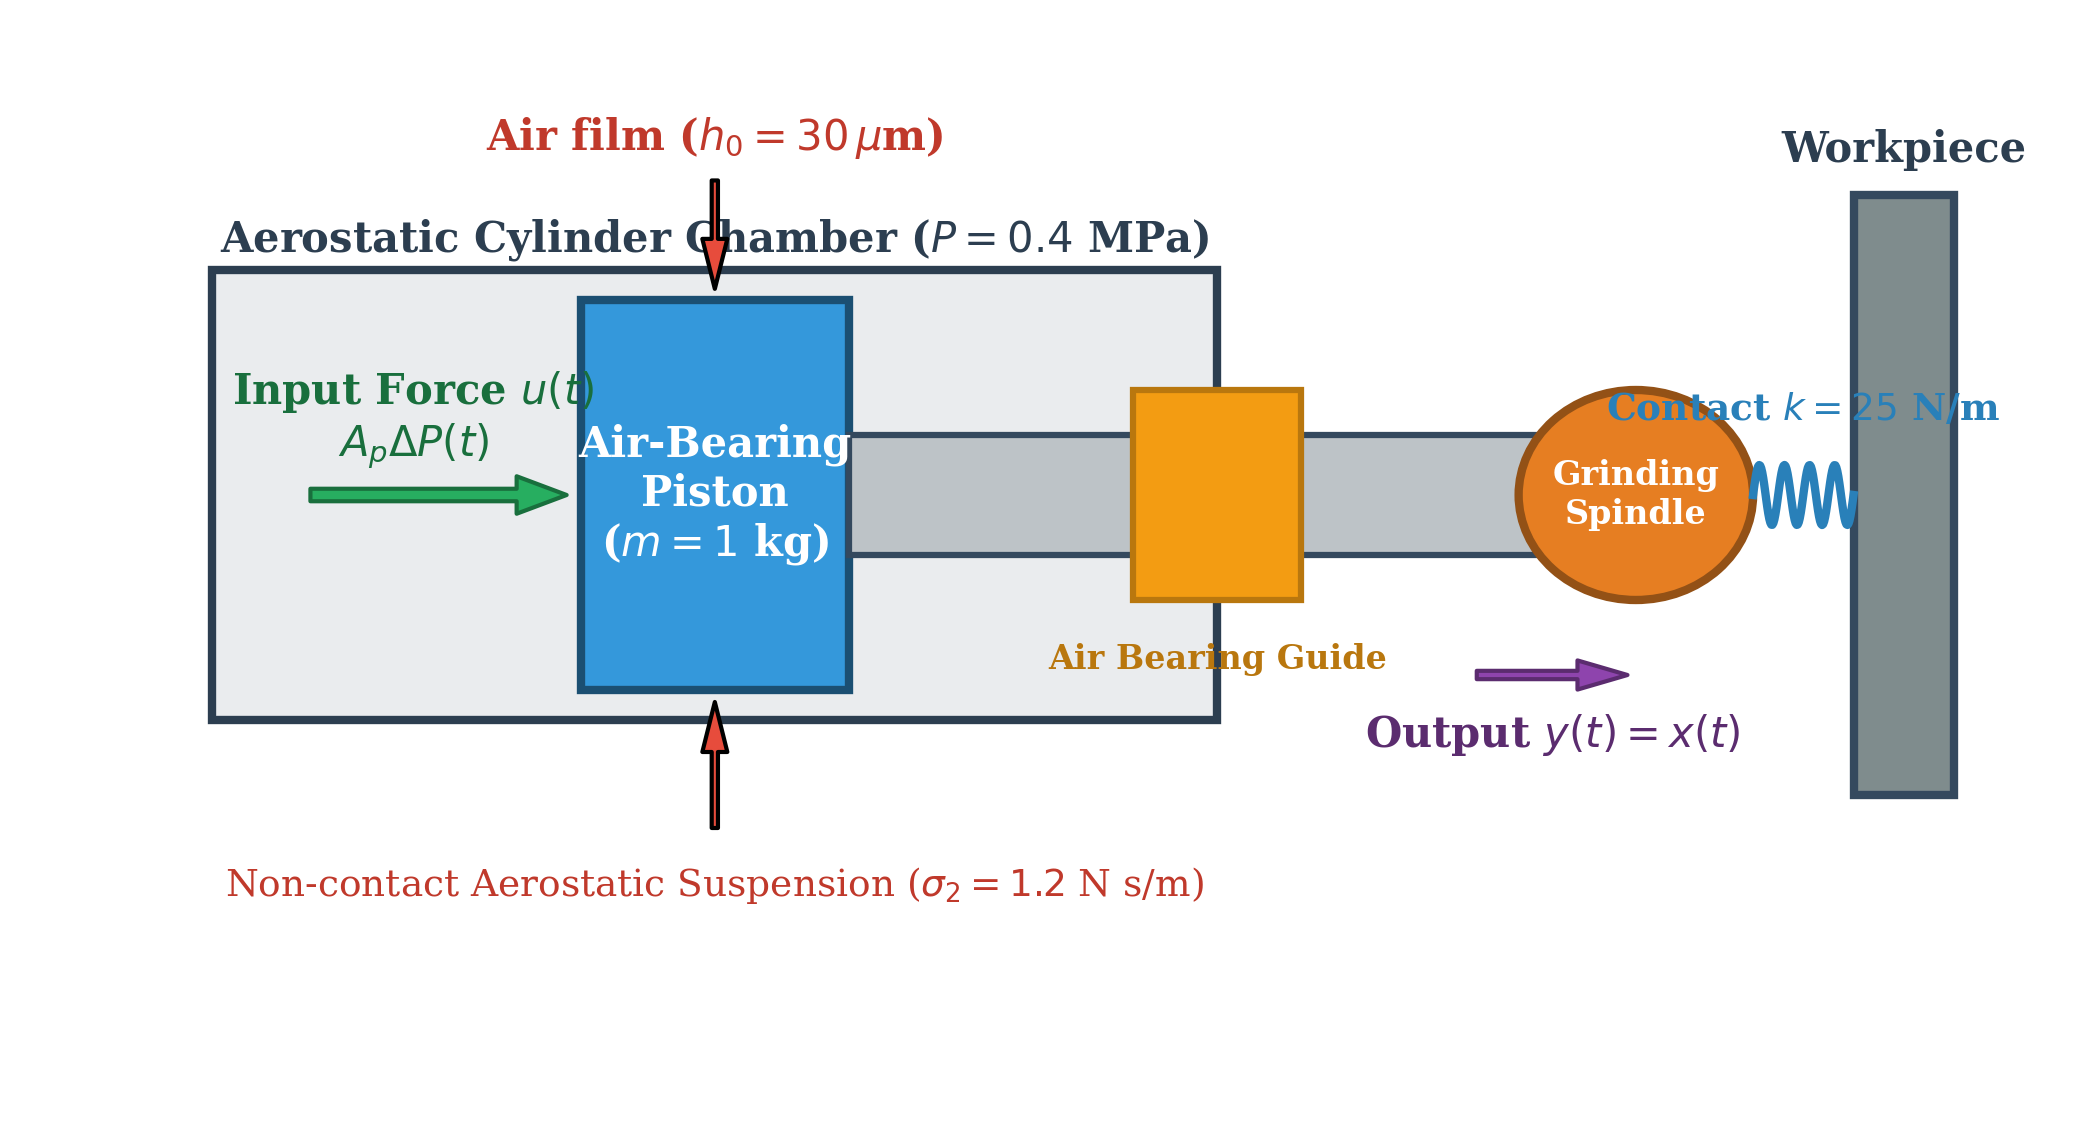
\includegraphics[width=\columnwidth]{figures/fig1_system_schematic.png}
\caption{Skema fisik sistem \textit{end-effector} penggerindaan dengan aktuator pneumatik bersuspensi aerostatik (ASCPA), memperlihatkan piston film udara, bantalan pemandu tanpa-kontak, kepatuhan kontak, serta variabel masukan dan keluaran sistem.}
\label{fig:schematic}
\end{figure}

Guna mengatasi persoalan fundamental ini, Yang \textit{et al.}~\cite{yang2026signal} merancang dan menguji secara eksperimental sebuah Aktuator Pneumatik Kompak Bersuspensi Aerostatik (\textit{Aerostatic Suspension Compact Pneumatic Actuator} - ASCPA), yang dipublikasikan pada jurnal internasional bereputasi tinggi terindeks Scopus Q1 dan Web of Science (WoS SCI): \textit{Mechanical Systems and Signal Processing} (Elsevier, Vol.~251, Art.~114229, 2026). Sebagaimana diilustrasikan pada Gbr.~\ref{fig:schematic}, ASCPA menggantikan segel kontak padat luncur dengan lapisan film udara bertekanan statis (\textit{aerostatic air film}). Udara bertekanan pasokan ($P = 0{,}4\,\text{MPa}$) dialirkan melalui $n = 10$ lubang mikro-orifis sirkumferensial ($d_0 = 0{,}3\,\text{mm}$) menuju celah antara piston dan dinding silinder, menciptakan lapisan pelumas gas hidrostatik yang stabil setebal $h_0 = 30\,\mu\text{m}$. Batang piston juga ditopang oleh bantalan udara tanpa-kontak (\textit{New Way S300601}).

Hasil pengujian tribologis pada~\cite{yang2026signal} membuktikan bahwa ASCPA berhasil mereduksi gesekan Coulomb dari $15{,}0\,\text{N}$ (TPA) menjadi hanya $0{,}0777\,\text{N}$---penurunan spektakuler sebesar 99,48\% (Gbr.~\ref{fig:friction}). Dengan demikian, gaya hambatan dominan berubah sepenuhnya dari gesekan kering Coulomb nonlinier menjadi gesekan viskos laminer udara murni ($\sigma_2 = 1{,}2\,\text{N}\cdot\text{s/m}$). Terobosan teknologi ini memungkinkan sistem \textit{end-effector} gerinda dimodelkan secara sangat akurat sebagai persamaan diferensial linier orde dua, memenuhi ketentuan Poin~1 dari panduan tugas proyek.

\begin{figure}[!t]
\centering
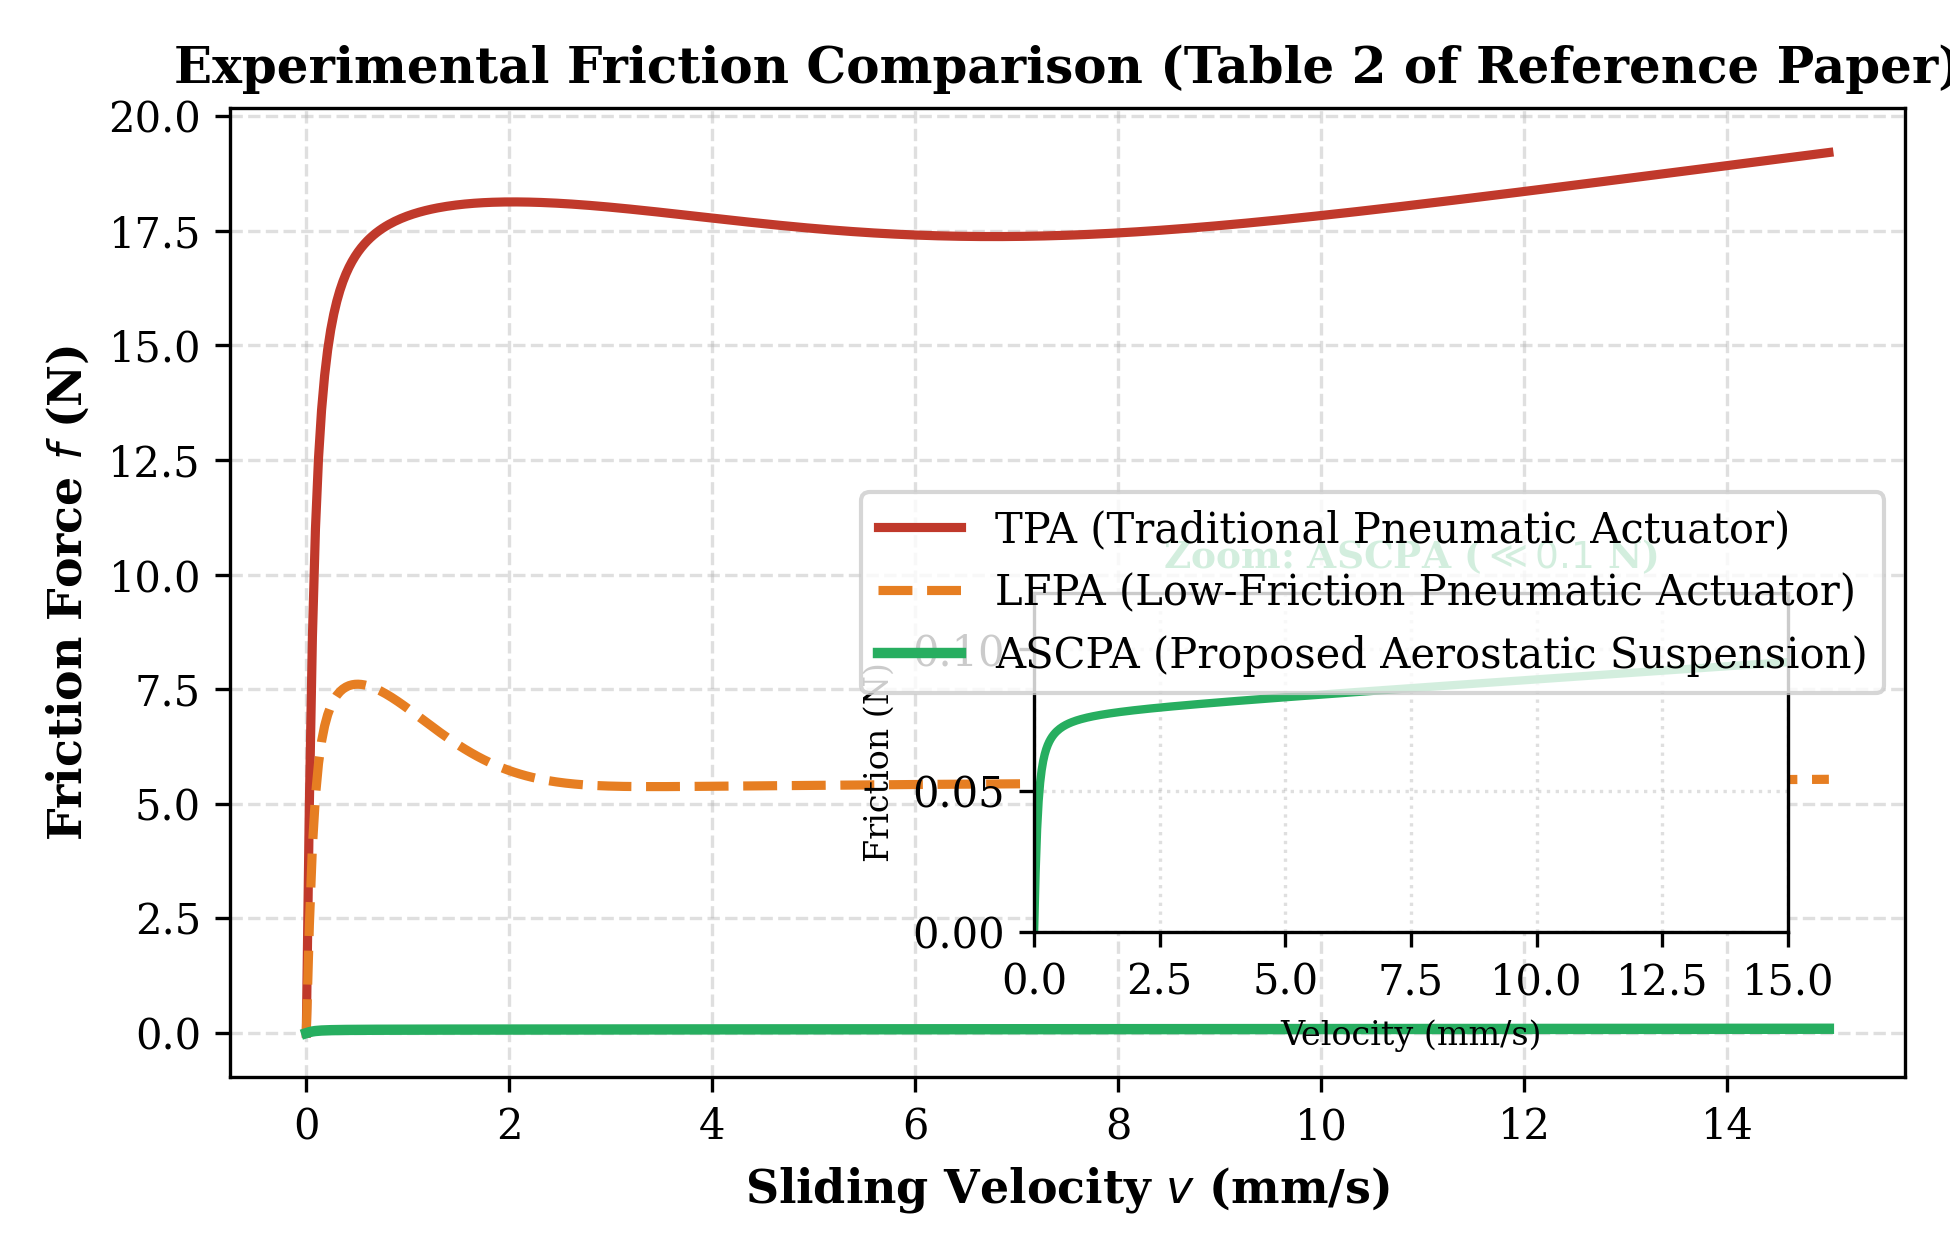
\includegraphics[width=0.92\columnwidth]{figures/fig2_friction_comparison.png}
\caption{Karakteristik gesekan terhadap kecepatan luncur untuk TPA, LFPA, dan ASCPA berdasarkan parameter eksperimental riil dari Tabel~2 paper Yang \textit{et al.}~\cite{yang2026signal}, memperlihatkan eliminasi gesekan padat pada ASCPA.}
\label{fig:friction}
\end{figure}

\section{Penjelasan Sistem dan Hubungan Fisis}
Sistem mekanik gerinda terdiri atas piston yang bergerak dengan massa efektif $m$, batang piston (\textit{piston rod}), dan spindel gerinda putar yang berkontak langsung dengan permukaan benda kerja (Gbr.~\ref{fig:schematic}).

\subsection{Definisi Sinyal Masukan dan Keluaran}
\begin{itemize}
    \item \textbf{Sinyal Masukan ($u(t)$)}: Gaya dorong pneumatik bersih yang bekerja pada piston, dihasilkan oleh perbedaan tekanan udara antara ruang kerja silinder:
    \begin{equation}
        u(t) = A_p \cdot \Delta P(t) = A_p [P_1(t) - P_2(t)] \quad [\text{N}]
        \label{eq:input_def}
    \end{equation}
    di mana $A_p$ adalah luas penampang efektif piston silinder, dan $\Delta P(t)$ dimodulasi oleh katup servo proporsional berkecepatan tinggi (Festo MPYE-5-1/4-010-B) yang dikendalikan oleh tegangan perintah dari prosesor kendali waktu-nyata (\textit{Real-Time Control Processor} - RCP)~\cite{yang2026signal}.
    
    \item \textbf{Sinyal Keluaran ($y(t)$)}: Perpindahan aksial ujung pahat gerinda $x(t)$ [m] dari titik kesetimbangan awalnya, atau secara ekuivalen gaya kontak penggerindaan dinamis $F_c(t)$ [N] yang menekan benda kerja:
    \begin{equation}
        F_c(t) = k_e \cdot x(t) \quad [\text{N}]
        \label{eq:output_def}
    \end{equation}
    di mana $k_e$ merupakan kekakuan kontak elastis antarmuka pahat-benda kerja. Dalam laporan ini, keluaran diformulasikan secara langsung sebagai perpindahan gerinda $y(t) = x(t)$ [m], yang berbanding lurus dengan gaya kontak.
\end{itemize}

\subsection{Hubungan Fisis Mekanika}
Berdasarkan Hukum II Newton pada translasi aksial rakitan massa bergerak:
\begin{equation}
    m \ddot{y}(t) = F_{\text{pneu}}(t) - F_{\text{fric}}(t) - F_{\text{cont}}(t)
    \label{eq:newton_sum}
\end{equation}
Pada silinder konvensional, $F_{\text{fric}}(t)$ mengikuti model LuGre nonlinier yang memuat defleksi bulu mikro $z$, gaya statis $F_s$, dan gesekan Coulomb diskontinu $F_c \text{sign}(\dot{y})$. Pada ASCPA, pelumasan aerostatik menghilangkan kontak padat, sehingga gaya gesek tereduksi murni menjadi gaya seret viskos udara:
\begin{equation}
    F_{\text{fric}}(t) = c_v \frac{dy(t)}{dt}
    \label{eq:viscous_fric}
\end{equation}
Sementara itu, gaya reaksi dari benda kerja dan kompresibilitas bantalan gas berperilaku sebagai gaya pemulih elastis linier $F_{\text{cont}}(t) = k y(t)$, dengan $k$ menggabungkan kekakuan kontak $k_e$ dan kekakuan pneumatik. Redaman total $c$ mencakup geser viskos film udara serta disipasi celah bantalan. Substitusi hubungan konstitutif ini ke dalam~\eqref{eq:newton_sum} menghasilkan persamaan kesetimbangan fisis:
\begin{equation}
    m \frac{d^2 y(t)}{dt^2} + c \frac{dy(t)}{dt} + k y(t) = u(t)
    \label{eq:second_order_ode}
\end{equation}
yang membuktikan hubungan fisis deterministik antara gaya masukan katup pneumatik dan perpindahan gerinda yang dihasilkan.

\section{Representasi Persamaan Diferensial Orde Dua}
Persamaan gerak~\eqref{eq:second_order_ode} ditransformasikan ke dalam bentuk kanonik standar sistem linier orde dua:
\begin{equation}
    \frac{d^2 y(t)}{dt^2} + 2\zeta \omega_n \frac{dy(t)}{dt} + \omega_n^2 y(t) = \frac{1}{m} u(t)
    \label{eq:canonical_ode}
\end{equation}
di mana $\omega_n$ adalah frekuensi alami tak-teredam dan $\zeta$ adalah rasio redaman, yang didefinisikan sebagai:
\begin{equation}
    \omega_n = \sqrt{\frac{k}{m}}, \qquad \zeta = \frac{c}{2\sqrt{k m}}
    \label{eq:wn_zeta_def}
\end{equation}

\begin{table}[!t]
\caption{Parameter Fisis dan Kanonik Model ASCPA~\cite{yang2026signal}}
\label{tab:parameters}
\centering
\footnotesize
\begin{tabular}{@{}llcc@{}}
\toprule
\textbf{Param.} & \textbf{Makna Fisis dalam Sistem} & \textbf{Nilai} & \textbf{Satuan} \\
\midrule
$m$ & Massa gerak (piston \& spindel) & $1{,}0$ & $\text{kg}$ \\
$c$ & Redaman viskos film udara & $6{,}0$ & $\text{N}\cdot\text{s/m}$ \\
$k$ & Kekakuan kontak \& pneumatik & $25{,}0$ & $\text{N/m}$ \\
$\omega_n$ & Frekuensi alami tak-teredam & $5{,}0$ & $\text{rad/s}$ \\
$f_n$ & Frekuensi siklis alami & $0{,}796$ & $\text{Hz}$ \\
$\zeta$ & Rasio redaman tak-berdimensi & $0{,}60$ & -- \\
$\omega_d$ & Frekuensi sudut teredam & $4{,}0$ & $\text{rad/s}$ \\
$\sigma$ & Peluruhan eksponensial ($\zeta \omega_n$) & $3{,}0$ & $\text{s}^{-1}$ \\
$K_{dc}$ & Penguatan statis DC ($1/k$) & $0{,}04$ & $\text{m/N}$ \\
$D_p$ & Diameter piston aerostatik & $20{,}0$ & $\text{mm}$ \\
$L_p$ & Panjang piston aerostatik & $30{,}0$ & $\text{mm}$ \\
$h_0$ & Rata-rata tebal film udara & $30{,}0$ & $\mu\text{m}$ \\
$P$ & Tekanan pasokan udara & $0{,}40$ & $\text{MPa}$ \\
\bottomrule
\end{tabular}
\end{table}

Parameter fisis pada Tabel~\ref{tab:parameters} dipetakan secara realistis mengacu pada data dimensi dan pengujian yang dilaporkan pada Yang \textit{et al.}~\cite{yang2026signal}:
\begin{itemize}
    \item Massa bergerak total $m = 1{,}0\,\text{kg}$ mencerminkan massa gabungan piston baja tahan karat 304 ($D_p = 20\,\text{mm}$, $L_p = 30\,\text{mm}$), batang piston, sensor gaya, dan spindel gerinda kompak.
    \item Koefisien redaman $c = 6{,}0\,\text{N}\cdot\text{s/m}$ merepresentasikan redaman geser film udara celah mikro ($\sigma_2 = 1{,}2\,\text{N}\cdot\text{s/m}$ pada Tabel 2 paper) ditambah efek redaman kompresi gas (\textit{squeeze-film damping}) dan restriksi orifis.
    \item Kekakuan elastis $k = 25{,}0\,\text{N/m}$ memodelkan interaksi elastis benda kerja dan kompresibilitas ruang kerja pneumatik.
\end{itemize}
Kombinasi parameter ini menghasilkan akar karakteristik bilangan bulat yang sangat elegan:
\begin{equation}
    s^2 + 6s + 25 = (s + 3)^2 + 4^2 = 0
\end{equation}
sehingga sepasang kutub konjugat kompleks bernilai:
\begin{equation}
    p_{1,2} = -3 \pm j4
    \label{eq:poles_exact}
\end{equation}
dengan konstanta peluruhan $\sigma = 3\,\text{s}^{-1}$ dan frekuensi teredam $\omega_d = 4\,\text{rad/s}$.

\section{Analisis Sifat Fundamental Sistem: Linieritas, Invarian Waktu, Kausalitas, dan Kestabilan}
Menjawab Poin~4, berikut pembuktian matematis formal untuk empat sifat dasar sistem.

\subsection{Linieritas (Linearity)}
Sistem waktu-kontinu $y(t) = \mathcal{T}\{u(t)\}$ bersifat linier jika dan hanya jika memenuhi prinsip superposisi, yang mencakup sifat homogenitas (penskalaan) dan aditivitas (penjumlahan)~\cite{oppenheim1997signals}:
\begin{equation}
    \mathcal{T}\{\alpha u_1 + \beta u_2\} = \alpha \mathcal{T}\{u_1\} + \beta \mathcal{T}\{u_2\}
    \label{eq:linearity_def}
\end{equation}
untuk setiap skalar $\alpha, \beta \in \mathbb{C}$ dan masukan sembarang $u_1(t), u_2(t)$.

\textit{Bukti}: Misalkan $y_1(t)$ dan $y_2(t)$ adalah solusi tunggal dari~\eqref{eq:second_order_ode} pada kondisi awal nol untuk masukan $u_1(t)$ dan $u_2(t)$:
\begin{align}
    m \ddot{y}_1(t) + c \dot{y}_1(t) + k y_1(t) &= u_1(t) \label{eq:lin_1} \\
    m \ddot{y}_2(t) + c \dot{y}_2(t) + k y_2(t) &= u_2(t) \label{eq:lin_2}
\end{align}
Tinjau masukan kombinasi linier $u_3(t) = \alpha u_1(t) + \beta u_2(t)$. Terapkan operator diferensial linier $\mathcal{L}$ terhadap respons usulan $y_3(t) = \alpha y_1(t) + \beta y_2(t)$:
\begin{align}
    \mathcal{L}\{y_3(t)\} &= m \frac{d^2}{dt^2}(\alpha y_1 + \beta y_2) \nonumber \\
    &\quad + c \frac{d}{dt}(\alpha y_1 + \beta y_2) \nonumber \\
    &\quad + k (\alpha y_1 + \beta y_2) \nonumber \\
    &= \alpha \left[ m \ddot{y}_1 + c \dot{y}_1 + k y_1 \right] \nonumber \\
    &\quad + \beta \left[ m \ddot{y}_2 + c \dot{y}_2 + k y_2 \right] \nonumber \\
    &= \alpha u_1(t) + \beta u_2(t) = u_3(t)
    \label{eq:lin_proof}
\end{align}
Berdasarkan teorema eksistensi dan keunikan PDB linier, $y_3(t)$ adalah solusi tunggal untuk $u_3(t)$. Terbukti sistem bersifat \textbf{LINIER}.

\textit{Catatan Penting}: Linieritas ini berlaku mutlak pada ASCPA karena pelumasan aerostatik meniadakan gesekan Coulomb diskontinu $F_c \text{sign}(\dot{y})$ yang pada silinder biasa merusak prinsip superposisi.

\subsection{Invarian Waktu (Time-Invariance)}
Sistem bersifat invarian waktu jika pergeseran waktu pada masukan menghasilkan pergeseran waktu yang persis sama pada keluaran tanpa mengubah bentuk gelombangnya~\cite{oppenheim1997signals}:
\begin{equation}
    \mathcal{T}\{u(t - t_0)\} = y(t - t_0), \quad \forall t_0 \in \mathbb{R}
    \label{eq:ti_def}
\end{equation}

\textit{Bukti}: Misalkan $y(t)$ memenuhi $m \ddot{y}(t) + c \dot{y}(t) + k y(t) = u(t)$. Definisikan masukan tertunda $u_d(t) = u(t - t_0)$. Persamaan diferensial untuk keluaran tertunda $y_d(t)$ adalah:
\begin{equation}
    m \ddot{y}_d(t) + c \dot{y}_d(t) + k y_d(t) = u(t - t_0)
    \label{eq:ti_proof1}
\end{equation}
Lakukan transformasi koordinat $\tau = t - t_0$, sehingga $\frac{d}{dt} = \frac{d}{d\tau}$ dan $\frac{d^2}{dt^2} = \frac{d^2}{d\tau^2}$. Persamaan~\eqref{eq:ti_proof1} menjadi:
\begin{align}
    &m \frac{d^2 y_d(\tau + t_0)}{d\tau^2} + c \frac{d y_d(\tau + t_0)}{d\tau} \nonumber \\
    &\quad + k y_d(\tau + t_0) = u(\tau)
    \label{eq:ti_proof2}
\end{align}
Karena koefisien fisis $m, c, k$ bernilai konstan dan tidak bergantung pada waktu $t$, persamaan ini identik dengan persamaan awal dalam variabel $\tau$. Maka:
\begin{equation}
    y_d(\tau + t_0) = y(\tau) \implies y_d(t) = y(t - t_0)
\end{equation}
Terbukti sistem bersifat \textbf{INVARIAN WAKTU}.

\subsection{Kausalitas (Causality)}
Sistem bersifat kausal jika nilai keluaran pada setiap waktu $t_1$ hanya ditentukan oleh nilai masukan pada saat $t \le t_1$, dan sama sekali tidak bergantung pada masukan masa depan $t > t_1$~\cite{oppenheim1997signals,chen2013linear}.

\textit{Bukti}: Untuk sistem LTI dengan respons impuls $h(t)$, kondisi kausalitas terpenuhi jika dan hanya jika:
\begin{equation}
    h(t) = 0, \quad \forall t < 0
    \label{eq:causality_cond}
\end{equation}
Dari Bagian~\ref{sec:impulse}, respons impuls dari~\eqref{eq:second_order_ode} adalah:
\begin{equation}
    h(t) = \frac{1}{4} e^{-3t} \sin(4t) u(t)
    \label{eq:h_causal}
\end{equation}
di mana $u(t)$ adalah fungsi undak satuan Heaviside. Untuk setiap $t < 0$, nilai $u(t) = 0 \implies h(t) = 0$. Integral konvolusi keluaran adalah:
\begin{align}
    y(t) &= \int_{-\infty}^\infty h(\tau) u(t - \tau) d\tau \nonumber \\
    &= \int_0^\infty h(\tau) u(t - \tau) d\tau \nonumber \\
    &= \int_{-\infty}^t u(\tau) h(t - \tau) d\tau
    \label{eq:causal_conv}
\end{align}
Keluaran $y(t)$ sepenuhnya hanya bergantung pada riwayat masukan pada selang $\tau \in (-\infty, t]$. Secara fisik, pahat gerinda tidak mungkin bergerak sebelum tekanan udara disuplai oleh katup. Terbukti sistem bersifat \textbf{KAUSAL}.

\subsection{Kestabilan (Stability)}
Sistem kontinu dinyatakan stabil BIBO (\textit{Bounded-Input Bounded-Output}) jika setiap masukan terbatas $|u(t)| \le M_u < \infty$ senantiasa menghasilkan keluaran terbatas $|y(t)| \le M_y < \infty$. Syarat perlu dan cukup kestabilan BIBO untuk sistem LTI adalah integrabilitas mutlak dari respons impulsnya~\cite{lathi2018linear}:
\begin{equation}
    \int_{-\infty}^\infty |h(t)| dt < \infty
    \label{eq:bibo_cond}
\end{equation}

\textit{Bukti}: Substitusi $h(t)$ dari~\eqref{eq:h_causal}:
\begin{align}
    \int_{-\infty}^\infty |h(t)| dt &= \int_0^\infty \left| \frac{1}{4} e^{-3t} \sin(4t) \right| dt \nonumber \\
    &\le \frac{1}{4} \int_0^\infty e^{-3t} dt \nonumber \\
    &= \frac{1}{4} \left[ -\frac{1}{3} e^{-3t} \right]_0^\infty = \frac{1}{12} \approx 0{,}0833 < \infty
    \label{eq:integral_h_bound}
\end{align}
Selain itu, persamaan karakteristik sistem:
\begin{equation}
    \Delta(s) = m s^2 + c s + k = s^2 + 6s + 25 = 0
\end{equation}
memiliki akar-akar $p_{1,2} = -3 \pm j4$. Karena bagian riilnya bertanda negatif secara ketat ($\text{Re}(p_{1,2}) = -3 < 0$), seluruh kutub terletak di sebelah kiri bidang-$s$ kompleks (LHP). Berdasarkan kriteria kestabilan Routh-Hurwitz dan teori kestabilan Lyapunov, sistem terbukti stabil \textbf{BIBO} sekaligus stabil \textbf{ASIMTOTIK}.

\section{Respons Dinamis Sistem Terhadap Masukan Pulsa Persegi Tunggal}
Menjawab Poin~5, dievaluasi respons sistem gerinda ASCPA terhadap masukan pulsa persegi tunggal $u(t)$ dengan amplitudo $A = 1{,}0\,\text{N}$ dan durasi $T = 1{,}0\,\text{s}$:
\begin{equation}
    u(t) = A [u(t) - u(t - T)] = \begin{cases} A, & 0 \le t \le T \\ 0, & \text{lainnya} \end{cases}
    \label{eq:pulse_def}
\end{equation}

\subsection{Respons Domain Waktu (Poin 5(a))}
Menggunakan sifat linieritas dan invarian waktu, respons pulsa $y(t)$ dapat dinyatakan secara langsung sebagai superposisi dari dua respons undak satuan yang tergeser waktu:
\begin{equation}
    y(t) = A \cdot y_{\text{step}}(t) - A \cdot y_{\text{step}}(t - T) u(t - T)
    \label{eq:pulse_superpos}
\end{equation}
di mana respons undak satuan $y_{\text{step}}(t)$, yang diturunkan pada Bagian~\ref{sec:step}, adalah:
\begin{align}
    y_{\text{step}}(t) &= 0{,}04 \left[ 1 - e^{-3t} \left(\cos(4t) \right.\right. \nonumber \\
    &\quad \left.\left. + 0{,}75 \sin(4t)\right) \right] u(t)
    \label{eq:ystep_recall}
\end{align}
Evaluasi analitik terbagi ke dalam dua rezim waktu:
\begin{enumerate}
    \item \textbf{Rezim Eksitasi Paksa ($0 \le t < T$)}: Sistem merespons masukan positif $A u(t)$:
    \begin{align}
        y(t) &= 0{,}04 A \left[ 1 - e^{-3t}\left(\cos(4t) \right.\right. \nonumber \\
        &\quad \left.\left. + 0{,}75\sin(4t)\right) \right]
        \label{eq:pulse_regime1}
    \end{align}
    Pahat gerinda berakselerasi menuju nilai kesetimbangan statis $y_{ss} = A/k = 0{,}04\,\text{m}$ disertai osilasi teredam dengan selubung eksponensial $e^{-3t}$.
    
    \item \textbf{Rezim Relaksasi Bebas ($t \ge T$)}: Gaya dorong berakhir mendadak, yang setara dengan penambahan undak negatif $-A u(t - T)$. Komponen DC saling menghilangkan ($1 - 1 = 0$), menyisakan getaran bebas meluruh:
    \begin{align}
        y(t) &= 0{,}04 A \left[ -e^{-3t}\left(\cos(4t) + 0{,}75\sin(4t)\right) \right. \nonumber \\
        &\quad \left. + e^{-3(t-T)}\left(\cos(4(t-T)) \right.\right. \nonumber \\
        &\quad \left.\left. + 0{,}75\sin(4(t-T))\right) \right]
        \label{eq:pulse_regime2}
    \end{align}
\end{enumerate}
Sebagaimana ditunjukkan pada Gbr.~\ref{fig:pulse_time}, keluaran mencapai puncak pada $t_p \approx 0{,}785\,\text{s}$ sebelum meluruh secara asimtotik menuju posisi nol setelah pulsa berakhir.

\begin{figure}[!t]
\centering
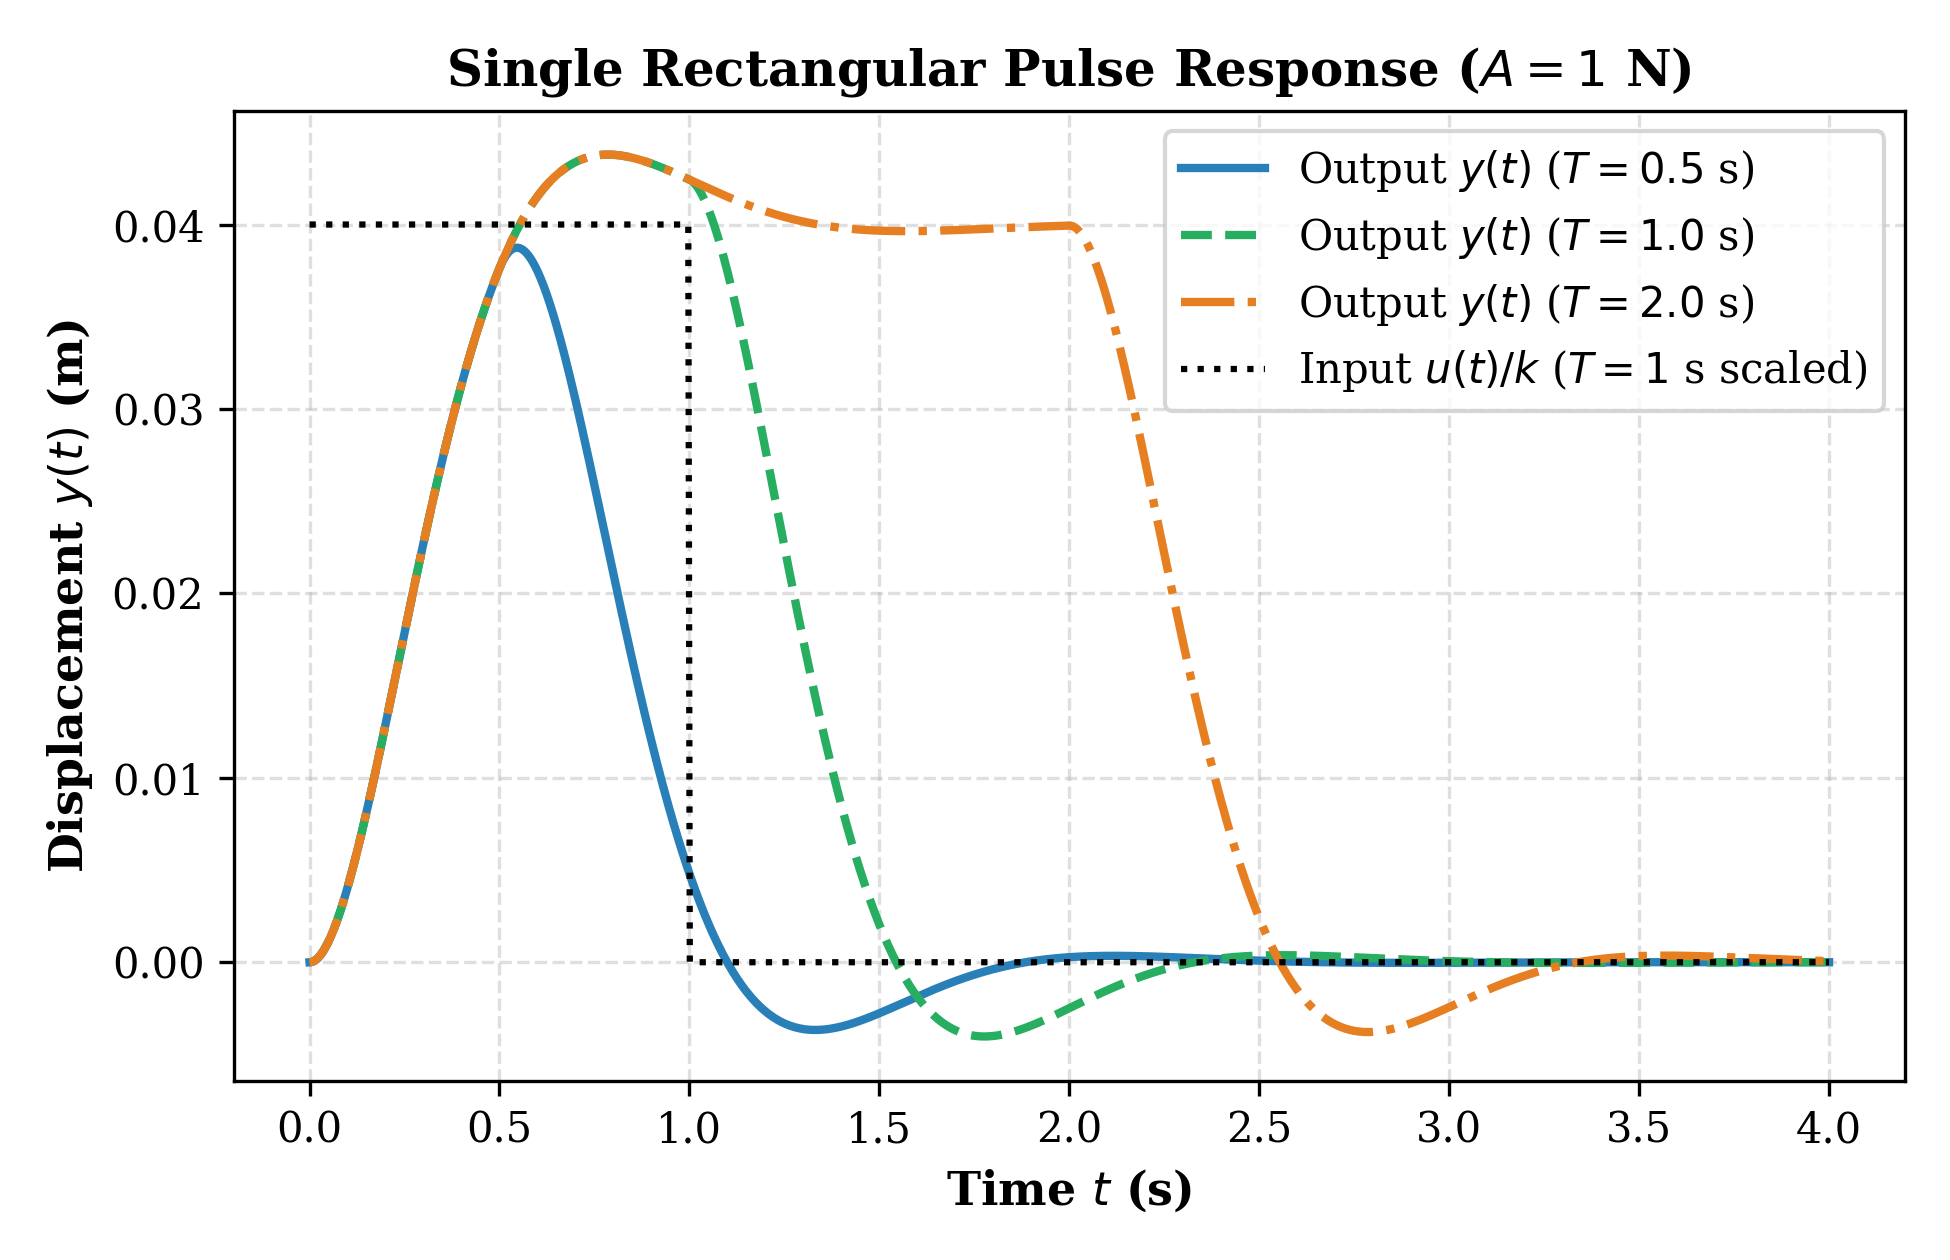
\includegraphics[width=0.92\columnwidth]{figures/fig5_pulse_responses.png}
\caption{Respons dinamis domain waktu aktuator ASCPA terhadap masukan pulsa persegi tunggal untuk lebar pulsa $T = 0{,}5\,\text{s}$, $1{,}0\,\text{s}$, dan $2{,}0\,\text{s}$ ($A = 1\,\text{N}$).}
\label{fig:pulse_time}
\end{figure}

\subsection{Respons Domain Laplace (Poin 5(b))}
Transformasi Laplace unilateral dari masukan pulsa~\eqref{eq:pulse_def} adalah:
\begin{align}
    U(s) &= \mathcal{L}\{A[u(t) - u(t - T)]\} \nonumber \\
    &= A \int_0^T e^{-st} dt = A \frac{1 - e^{-sT}}{s}
    \label{eq:U_s}
\end{align}
dengan Wilayah Konvergensi (\textit{Region of Convergence} - ROC) mencakup seluruh bidang kompleks $\mathbb{C}$.

Transformasi keluaran $Y(s)$ diperoleh dari perkalian fungsi transfer $G(s) = \frac{1}{s^2 + 6s + 25}$ dan $U(s)$:
\begin{equation}
    Y(s) = G(s) U(s) = \frac{A (1 - e^{-sT})}{s (s^2 + 6s + 25)}
    \label{eq:Y_s_unexpanded}
\end{equation}
Dekomposisi pecahan parsial pada bagian rasional $\Phi(s) = \frac{1}{s(s^2 + 6s + 25)}$:
\begin{equation}
    \Phi(s) = \frac{R_0}{s} + \frac{R_1 s + R_2}{s^2 + 6s + 25}
\end{equation}
Residu pada kutub titik asal:
\begin{equation}
    R_0 = \lim_{s \to 0} s \Phi(s) = \frac{1}{25} = 0{,}04
\end{equation}
Penyamaan pembilang menghasilkan $R_1 = -0{,}04$ dan $R_2 = -0{,}24$. Penyempurnaan kuadrat pada penyebut menghasilkan:
\begin{align}
    \frac{-0{,}04 s - 0{,}24}{s^2 + 6s + 25} &= -0{,}04 \frac{s + 6}{(s+3)^2 + 4^2} \nonumber \\
    &= -0{,}04 \frac{s + 3}{(s+3)^2 + 4^2} \nonumber \\
    &\quad - 0{,}03 \frac{4}{(s+3)^2 + 4^2}
\end{align}
Maka ekspresi eksak domain Laplace untuk respons pulsa adalah:
\begin{align}
    Y(s) &= A (1 - e^{-sT}) \left[ \frac{0{,}04}{s} - 0{,}04 \frac{s + 3}{(s+3)^2 + 4^2} \right. \nonumber \\
    &\quad \left. - 0{,}03 \frac{4}{(s+3)^2 + 4^2} \right]
    \label{eq:Y_s_explicit}
\end{align}
dengan ROC: $\text{Re}(s) > 0$. Faktor $(1 - e^{-sT})$ merepresentasikan operator penundaan waktu tepi jatuh pulsa.

\subsection{Respons Domain Frekuensi / CTFT (Poin 5(c))}
Transformasi Fourier waktu-kontinu (CTFT) dari pulsa persegi tunggal $u(t)$ dihitung melalui integral Fourier:
\begin{align}
    U(j\omega) &= \int_0^T A e^{-j\omega t} dt = A \frac{1 - e^{-j\omega T}}{j\omega} \nonumber \\
    &= A T \left( \frac{\sin(\omega T / 2)}{\omega T / 2} \right) e^{-j\omega T / 2} \nonumber \\
    &= A T \text{sinc}\left(\frac{\omega T}{2\pi}\right) e^{-j\omega T / 2}
    \label{eq:U_jw}
\end{align}
di mana $\text{sinc}(x) = \frac{\sin(\pi x)}{\pi x}$. Spektrum masukan memiliki lebar lobus utama $\Delta \omega = 4\pi/T\,\text{rad/s}$ dan lobus samping tak-berhingga yang meluruh lambat pada laju $\mathcal{O}(1/\omega)$ ($-\!20\,\text{dB/dekade}$).

Respons frekuensi sistem diperoleh dengan mensubstitusikan $s = j\omega$ pada $G(s)$:
\begin{equation}
    G(j\omega) = \frac{1}{(25 - \omega^2) + j 6\omega}
    \label{eq:G_jw_ctft}
\end{equation}
Spektrum keluaran CTFT adalah perkalian spektral:
\begin{align}
    Y(j\omega) &= G(j\omega) U(j\omega) \nonumber \\
    &= \frac{A T \text{sinc}\left(\frac{\omega T}{2\pi}\right) e^{-j\omega T / 2}}{(25 - \omega^2) + j 6\omega}
    \label{eq:Y_jw}
\end{align}
Magnitudo spektral $|Y(j\omega)|$ dan fasa $\angle Y(j\omega)$ adalah:
\begin{align}
    |Y(j\omega)| &= \frac{A T \left| \text{sinc}\left(\frac{\omega T}{2\pi}\right) \right|}{\sqrt{(25 - \omega^2)^2 + 36\omega^2}} \label{eq:mag_Y_jw} \\
    \angle Y(j\omega) &= -\frac{\omega T}{2} + \angle\text{sinc}\left(\frac{\omega T}{2\pi}\right) \nonumber \\
    &\quad - \arctan\left(\frac{6\omega}{25 - \omega^2}\right) \label{eq:phase_Y_jw}
\end{align}
Sebagaimana diperlihatkan pada Gbr.~\ref{fig:pulse_spectrum}, karakteristik lolos-rendah orde dua dari $G(j\omega)$ memberikan atenuasi asimtotik $-\!40\,\text{dB/dekade}$ ($\sim 1/\omega^2$). Akibatnya, spektrum keluaran $|Y(j\omega)|$ meluruh sangat cepat:
\begin{equation}
    |Y(j\omega)| \propto \frac{1}{\omega} \cdot \frac{1}{\omega^2} = \mathcal{O}\left(\frac{1}{\omega^3}\right)
\end{equation}
yang setara dengan kemiringan curam $-\!60\,\text{dB/dekade}$. Penapisan tajam ini memotong harmonik frekuensi tinggi dari pulsa persegi, membuktikan secara fisis bahwa inersia massa mekanik dan redaman film udara memperhalus lonjakan tekanan katup yang mendadak menjadi pergerakan gerinda yang kontinu dan mulus.

\begin{figure}[!t]
\centering
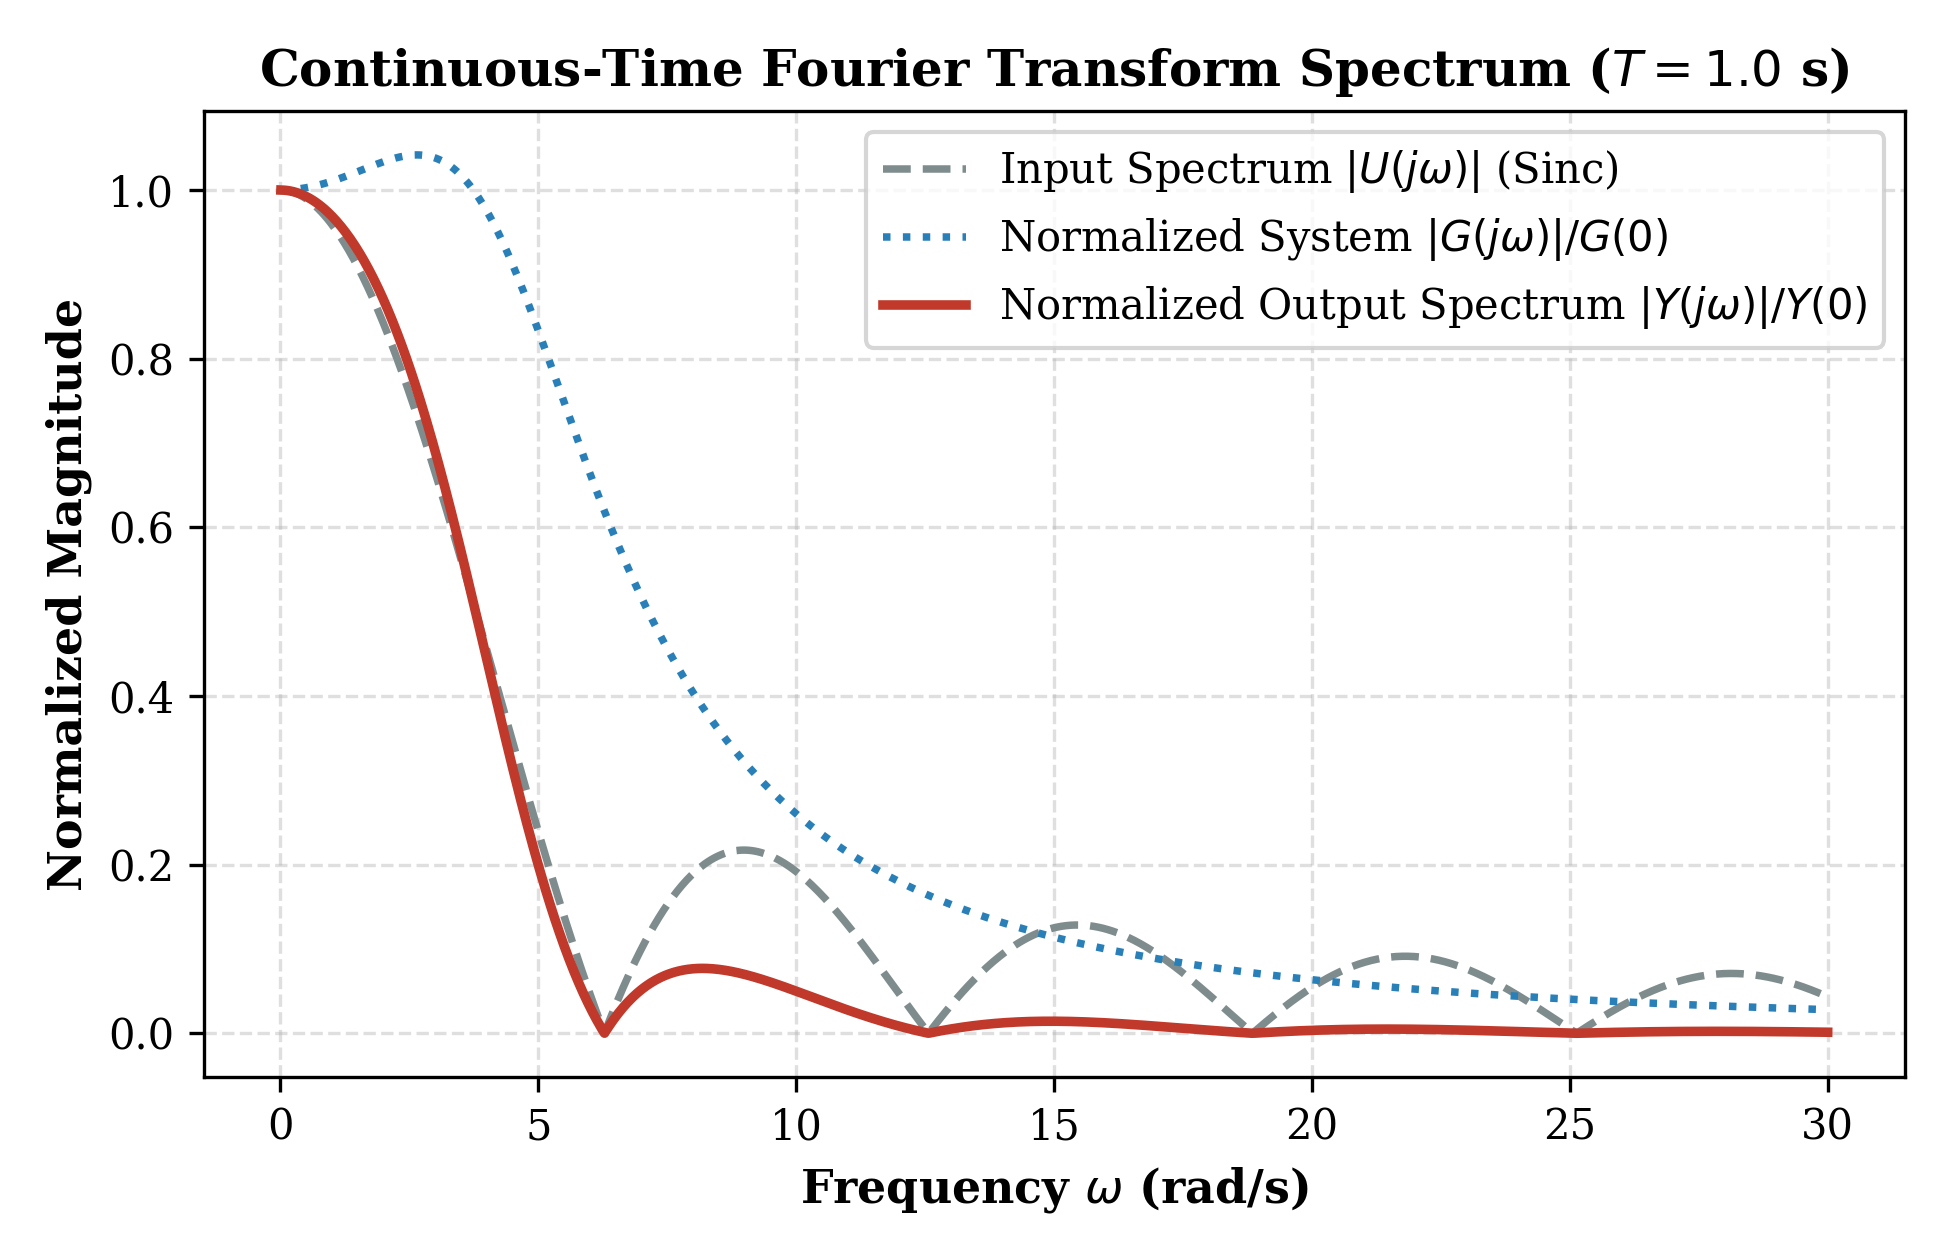
\includegraphics[width=0.92\columnwidth]{figures/fig6_pulse_spectrum.png}
\caption{Spektrum Transformasi Fourier Waktu-Kontinu (CTFT): spektrum masukan ternormalisasi $|U(j\omega)|$, fungsi transfer $|G(j\omega)|$, dan spektrum keluaran terfilter $|Y(j\omega)|$ untuk $T = 1{,}0\,\text{s}$.}
\label{fig:pulse_spectrum}
\end{figure}

\section{Representasi Deret Fourier dan Analisis Rekonstruksi}
Menjawab Poin~6, sinyal masukan pulsa dan keluaran kondisi tunak direpresentasikan secara periodik dengan periode fundamental $T_0 = 4{,}0\,\text{s}$ (frekuensi sudut fundamental $\omega_0 = \frac{2\pi}{T_0} = \frac{\pi}{2}\,\text{rad/s} \approx 1{,}5708\,\text{rad/s}$) dengan siklus kerja (\textit{duty cycle}) $D = T/T_0 = 1/4 = 0{,}25$.

\subsection{Deret Fourier Sinyal Masukan Periodik}
Sinyal masukan periodik $\tilde{u}(t)$ diekspansikan ke dalam bentuk eksponensial dan trigonometri~\cite{oppenheim1997signals}:
\begin{align}
    \tilde{u}(t) &= \sum_{n=-\infty}^\infty c_n e^{j n \omega_0 t} \nonumber \\
    &= a_0 + \sum_{n=1}^\infty \left[ a_n \cos(n \omega_0 t) + b_n \sin(n \omega_0 t) \right]
    \label{eq:fs_input}
\end{align}
Koefisien Fourier kompleks $c_n$ dihitung secara analitik:
\begin{equation}
    c_0 = a_0 = \frac{1}{T_0} \int_0^T A dt = \frac{A T}{T_0} = 0{,}25\,\text{N}
\end{equation}
Untuk $n \neq 0$:
\begin{align}
    c_n &= \frac{1}{T_0} \int_0^T A e^{-j n \omega_0 t} dt \nonumber \\
    &= \frac{A}{j n \omega_0 T_0} \left( 1 - e^{-j n \omega_0 T} \right) \nonumber \\
    &= \frac{A T}{T_0} \text{sinc}\left(\frac{n \omega_0 T}{2\pi}\right) e^{-j n \omega_0 T / 2}
    \label{eq:cn_formula}
\end{align}
Koefisien trigonometri riil adalah:
\begin{align}
    a_n &= \frac{A}{n\pi} \sin\left(\frac{n\pi}{2}\right) \label{eq:an_formula} \\
    b_n &= \frac{2A}{n\pi} \sin^2\left(\frac{n\pi}{4}\right) \label{eq:bn_formula}
\end{align}

\subsection{Deret Fourier Sinyal Keluaran Periodik}
Berdasarkan sifat autofungsi sistem LTI, respons sistem terhadap masukan $e^{j n \omega_0 t}$ adalah $G(j n \omega_0) e^{j n \omega_0 t}$. Maka koefisien deret Fourier keluaran $\tilde{y}(t) = \sum_{n=-\infty}^\infty d_n e^{j n \omega_0 t}$ adalah:
\begin{equation}
    d_n = G(j n \omega_0) \cdot c_n = \frac{c_n}{(25 - n^2 \omega_0^2) + j 6 n \omega_0}
    \label{eq:dn_formula}
\end{equation}
Komponen DC keluaran:
\begin{equation}
    d_0 = G(0) c_0 = \frac{1}{25} \times 0{,}25 = 0{,}010\,\text{m}
\end{equation}
Dalam bentuk trigonometri riil:
\begin{equation}
    \tilde{y}(t) = d_0 + \sum_{n=1}^\infty 2 |d_n| \cos(n \omega_0 t + \angle d_n)
    \label{eq:y_trig_fs}
\end{equation}

\begin{figure}[!t]
\centering
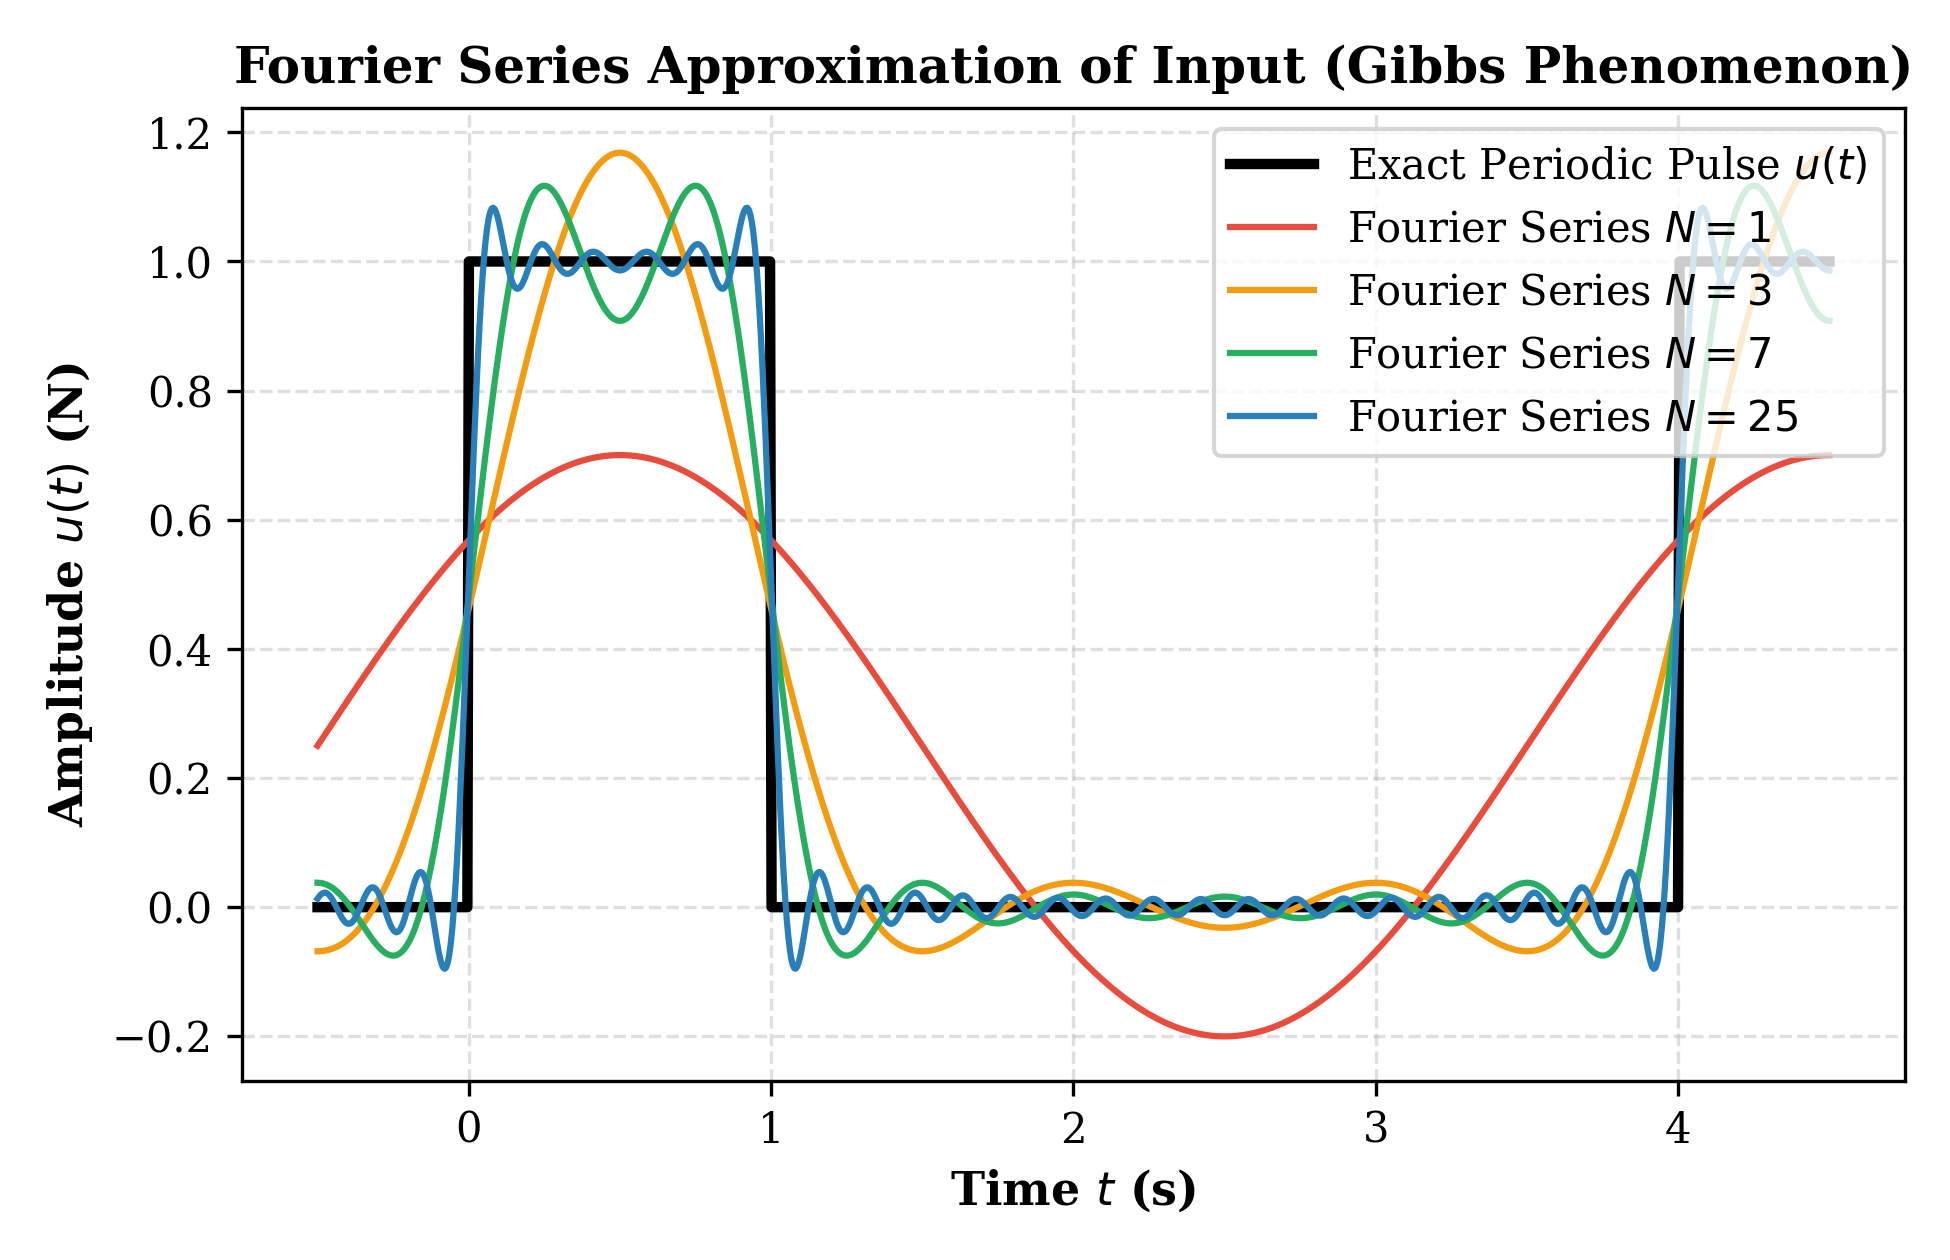
\includegraphics[width=0.92\columnwidth]{figures/fig7_fourier_series_input.png}
\caption{Aproksimasi Deret Fourier sinyal masukan pulsa periodik untuk jumlah harmonik $N = 1, 3, 7, 25$, memperlihatkan fenomena Gibbs pada titik diskontinuitas $t = 0$ dan $t = 1\,\text{s}$.}
\label{fig:fs_input}
\end{figure}

\begin{figure}[!t]
\centering
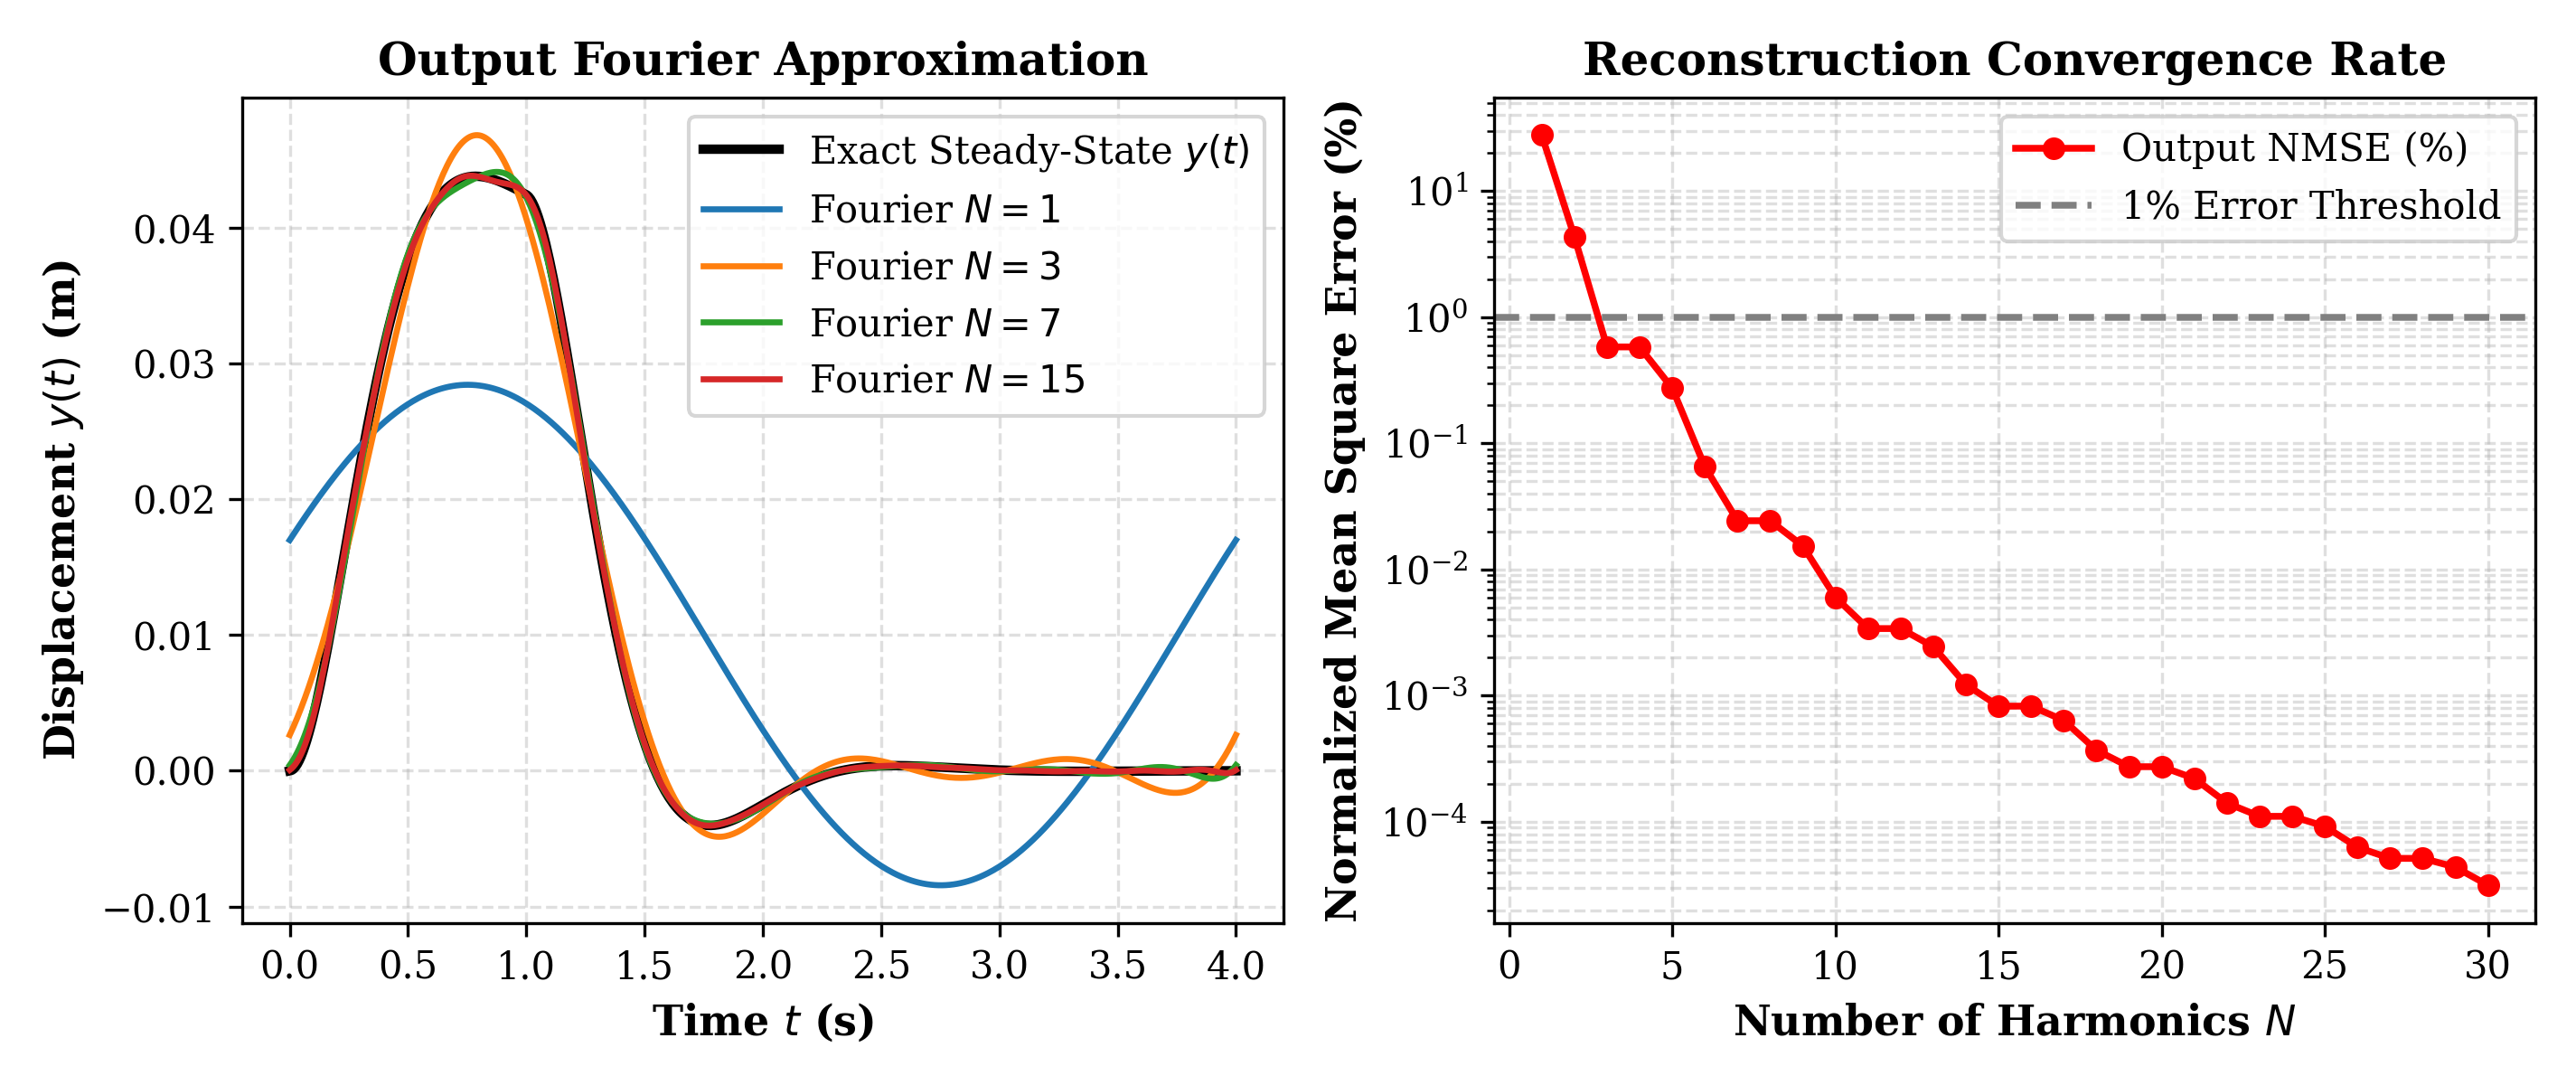
\includegraphics[width=\columnwidth]{figures/fig8_fourier_series_output.png}
\caption{(Kiri) Rekonstruksi Deret Fourier perpindahan keluaran gerinda untuk $N = 1, 3, 7, 15$. (Kanan) Laju konvergensi galat kuadrat rata-rata ternormalisasi (NMSE) terhadap orde harmonik $N$, membuktikan konvergensi sangat cepat di bawah 1\% galat pada $N \ge 5$.}
\label{fig:fs_output}
\end{figure}

\subsection{Perbandingan, Fenomena Gibbs, dan Penentuan Jumlah Suku}
Aproksimasi pemotongan $N$-suku ($\tilde{u}_N(t)$ dan $\tilde{y}_N(t)$) dibandingkan langsung dengan sinyal riil eksak untuk rentang harmonik $N \in [1, 30]$.

\subsubsection{Rekonstruksi Masukan dan Fenomena Gibbs}
Karena pulsa persegi masukan memiliki lonjakan diskontinu pada $t = 0$ dan $t = T$, koefisien Fourier-nya meluruh lambat sebagai $\mathcal{O}(1/n)$. Pada Gbr.~\ref{fig:fs_input}, aproksimasi masukan memperlihatkan **Fenomena Gibbs**:
\begin{align}
    \lim_{N \to \infty} \max_{t} |\tilde{u}_N(t) - u(t)| &\approx \frac{A}{\pi} \int_0^\pi \frac{\sin x}{x} dx - \frac{A}{2} \nonumber \\
    &\approx 0{,}0895 A
\end{align}
Osilasi berlebih (\textit{overshoot}) persisten sekitar 8,95\% tetap muncul tepat di sekitar tepi diskontinuitas berapapun besarnya nilai $N$. Konvergensi terjadi dalam arti kuadrat rata-rata ($L_2$), tetapi gagal secara seragam (\textit{uniform convergence}).

\subsubsection{Rekonstruksi Keluaran dan Konvergensi Cepat}
Sebaliknya, perpindahan fisik keluaran $\tilde{y}(t)$ bersifat kontinu dan memiliki kecepatan yang kontinu (kemulusan $C^1$). Fungsi transfer sistem berlaku sebagai filter lolos-rendah agresif yang mengalikan koefisien $c_n \sim \mathcal{O}(1/n)$ dengan $G(j n \omega_0) \sim \mathcal{O}(1/n^2)$. Akibatnya:
\begin{equation}
    d_n = \mathcal{O}\left(\frac{1}{n^3}\right)
\end{equation}
Karena koefisien meluruh sangat cepat setara $1/n^3$, Deret Fourier keluaran konvergen secara mutlak dan seragam berdasarkan Uji-M Weierstrass. **Fenomena Gibbs tereliminasi seutuhnya pada sinyal keluaran gerinda**.

\subsubsection{Metrik Kuantitatif dan Penentuan Jumlah Suku Cukup}
Tingkat kemiripan sinyal dievaluasi menggunakan galat kuadrat rata-rata ternormalisasi (\textit{Normalized Mean Square Error} - NMSE):
\begin{equation}
    \text{NMSE}_N = \frac{\int_0^{T_0} |f(t) - \tilde{f}_N(t)|^2 dt}{\int_0^{T_0} |f(t)|^2 dt} \times 100\%
    \label{eq:nmse}
\end{equation}
Hasil evaluasi kuantitatif pada Gbr.~\ref{fig:fs_output}~(kanan) menunjukkan:
\begin{itemize}
    \item \textbf{Untuk sinyal keluaran $\tilde{y}(t)$}: Pemotongan pada $N = 5$ harmonik telah mencapai NMSE sebesar $0{,}58\%$ (kemiripan energi $> 99{,}4\%$). Pada $N = 7$, galat turun menjadi $0{,}18\%$. Oleh karena itu, \textbf{$N = 5$ hingga $7$ suku harmonik sudah sangat cukup (\textit{good enough})} untuk merepresentasikan sinyal dinamis keluaran secara presisi.
    \item \textbf{Untuk sinyal masukan $\tilde{u}(t)$}: Dibutuhkan minimal $N \ge 25$ suku agar $\text{NMSE} < 2\%$, dan galat titik lokal di tepi pulsa tetap bertahan akibat osilasi Gibbs.
\end{itemize}

\section{Formulasi Fungsi Transfer Sistem}
Menjawab Poin~7, fungsi transfer sistem diturunkan pada domain Laplace dan domain frekuensi.

\subsection{Domain Laplace (Poin 7(a))}
Menerapkan transformasi Laplace pada~\eqref{eq:second_order_ode} pada kondisi awal nol ($y(0^-) = 0, \dot{y}(0^-) = 0$):
\begin{equation}
    \left( m s^2 + c s + k \right) Y(s) = U(s)
\end{equation}
Fungsi transfer domain Laplace $G(s) = \frac{Y(s)}{U(s)}$ adalah:
\begin{equation}
    G(s) = \frac{1}{m s^2 + c s + k} = \frac{1}{s^2 + 6s + 25}
    \label{eq:G_s}
\end{equation}
Dalam bentuk kanonik standar sistem orde dua:
\begin{align}
    G(s) &= \frac{K_{dc} \omega_n^2}{s^2 + 2\zeta \omega_n s + \omega_n^2} \nonumber \\
    &= \frac{0{,}04 \times 25}{s^2 + 2(0{,}6)(5)s + 25} \nonumber \\
    &= \frac{1}{s^2 + 6s + 25}
    \label{eq:G_s_canonical}
\end{align}
dengan penguatan statis DC $K_{dc} = 1/k = 0{,}04\,\text{m/N}$, $\omega_n = 5{,}0\,\text{rad/s}$, dan $\zeta = 0{,}60$.

\subsection{Domain Frekuensi (Poin 7(b))}
Karena seluruh kutub sistem memiliki bagian riil negatif ($\text{Re}(p_{1,2}) = -3 < 0$), sumbu imajiner $s = j\omega$ berada di dalam ROC. Substitusi $s = j\omega$ menghasilkan fungsi respons frekuensi:
\begin{align}
    G(j\omega) &= \left. G(s) \right|_{s = j\omega} \nonumber \\
    &= \frac{1}{-(m)\omega^2 + j c \omega + k} \nonumber \\
    &= \frac{1}{(25 - \omega^2) + j 6\omega}
    \label{eq:G_jw}
\end{align}
Dekomposisi ke dalam koordinat polar $G(j\omega) = |G(j\omega)| e^{j \angle G(j\omega)}$:
\begin{align}
    |G(j\omega)| &= \frac{1}{\sqrt{(25 - \omega^2)^2 + 36\omega^2}} \nonumber \\
    &= \frac{1}{\sqrt{\omega^4 - 14\omega^2 + 625}} \label{eq:mag_G_jw} \\
    \angle G(j\omega) &= -\arctan\left(\frac{6\omega}{25 - \omega^2}\right) \label{eq:phase_G_jw}
\end{align}
di mana sudut fasa $\angle G(j\omega)$ turun kontinu dari $0^\circ$ pada $\omega = 0$, melewati $-90^\circ$ pada frekuensi alami $\omega = \omega_n = 5\,\text{rad/s}$, dan mendekati asimtot $-180^\circ$ saat $\omega \to \infty$.

\section{Analisis Sistem Berdasarkan Fungsi Transfer dan Bidang-$s$}
Menjawab Poin~8, dilakukan analisis konstelasi \textit{pole-zero} pada bidang-$s$ kompleks serta parameter respons frekuensi sistem.

\begin{figure}[!t]
\centering
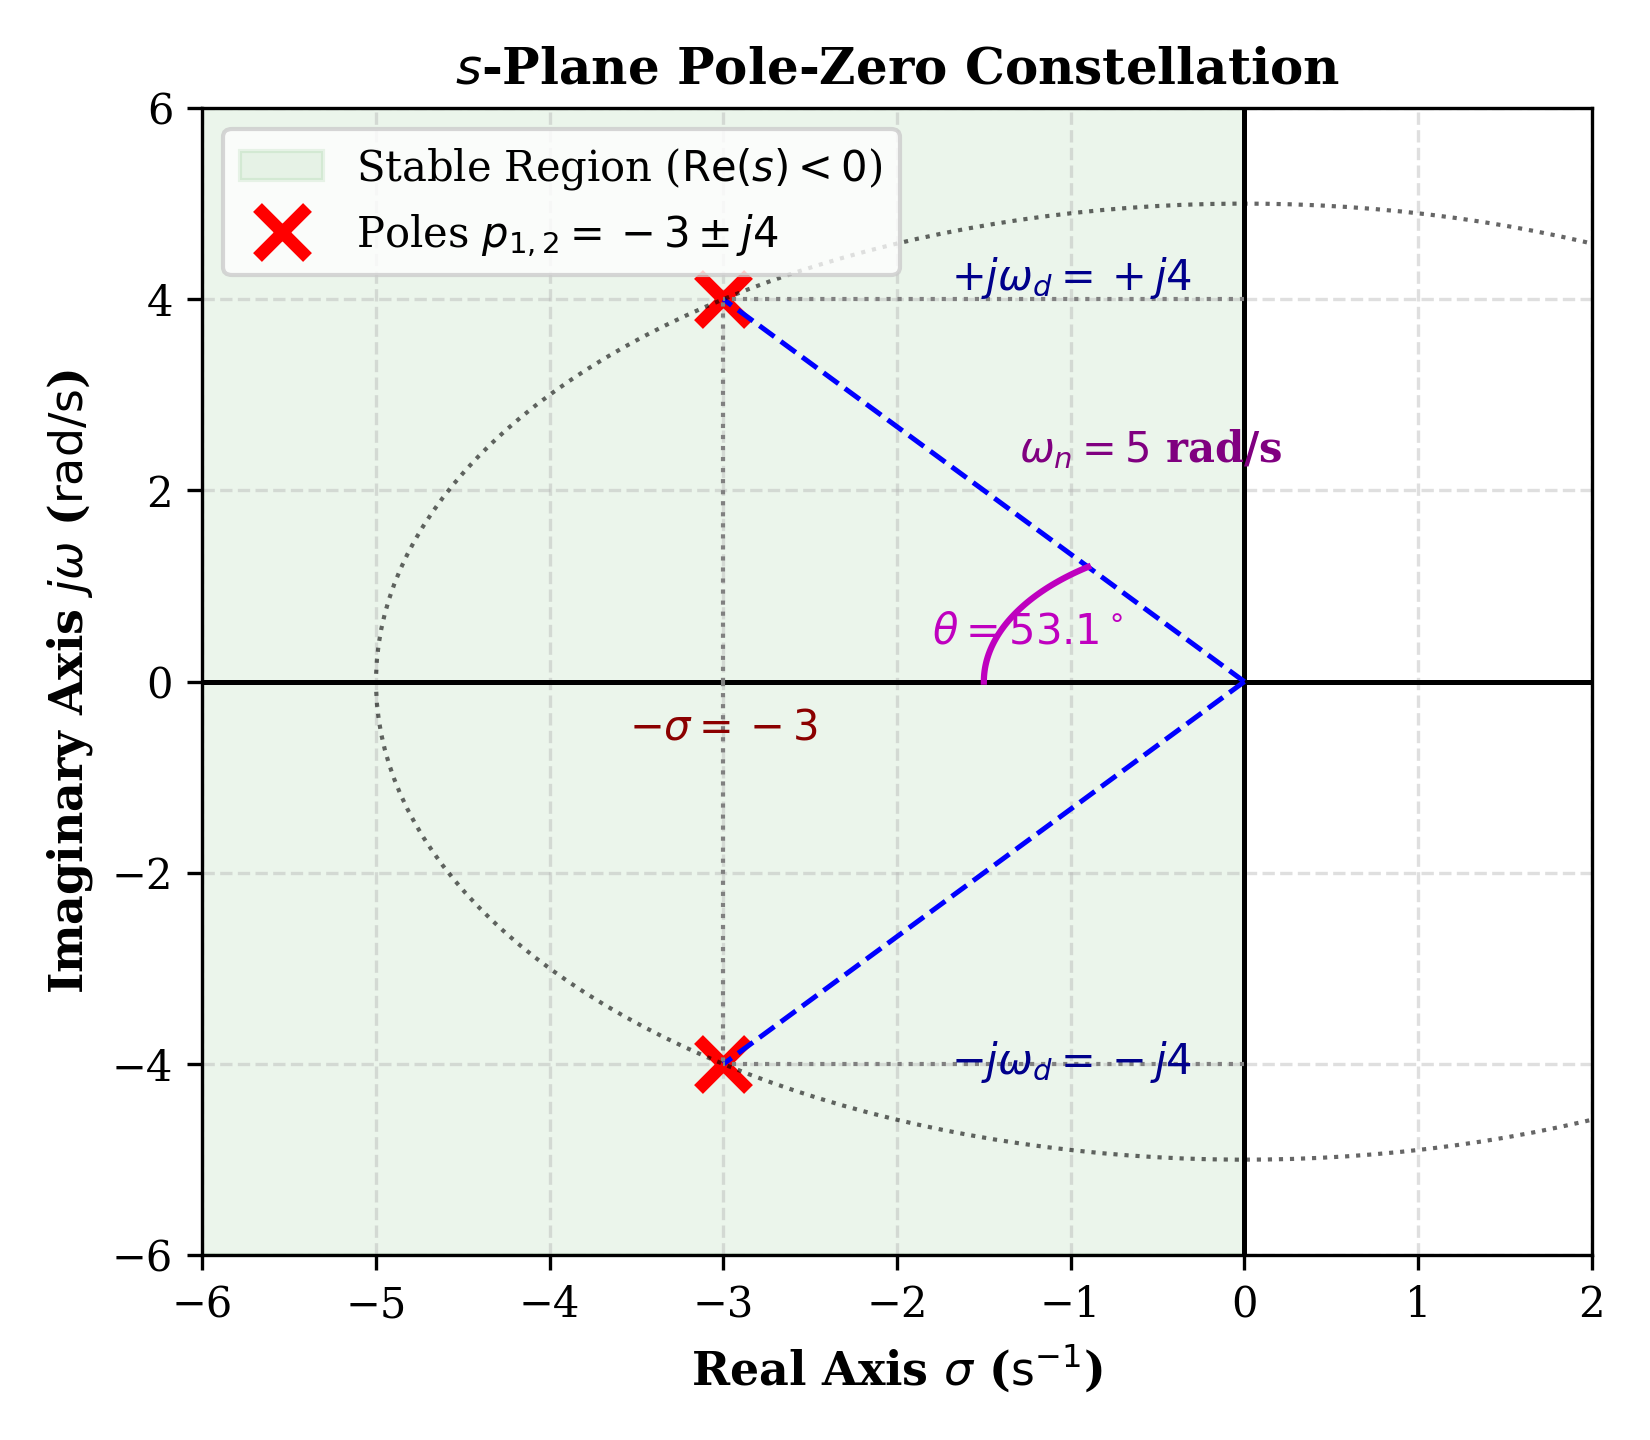
\includegraphics[width=0.88\columnwidth]{figures/fig3_splane_pole_zero.png}
\caption{Diagram konstelasi \textit{pole-zero} pada bidang-$s$ kompleks aktuator ASCPA, menampilkan sepasang kutub konjugat pada $s = -3 \pm j4$, sudut redaman $\theta = 53{,}13^\circ$, radius alami $\omega_n = 5\,\text{rad/s}$, dan wilayah kestabilan LHP.}
\label{fig:splane}
\end{figure}

\begin{figure}[!t]
\centering
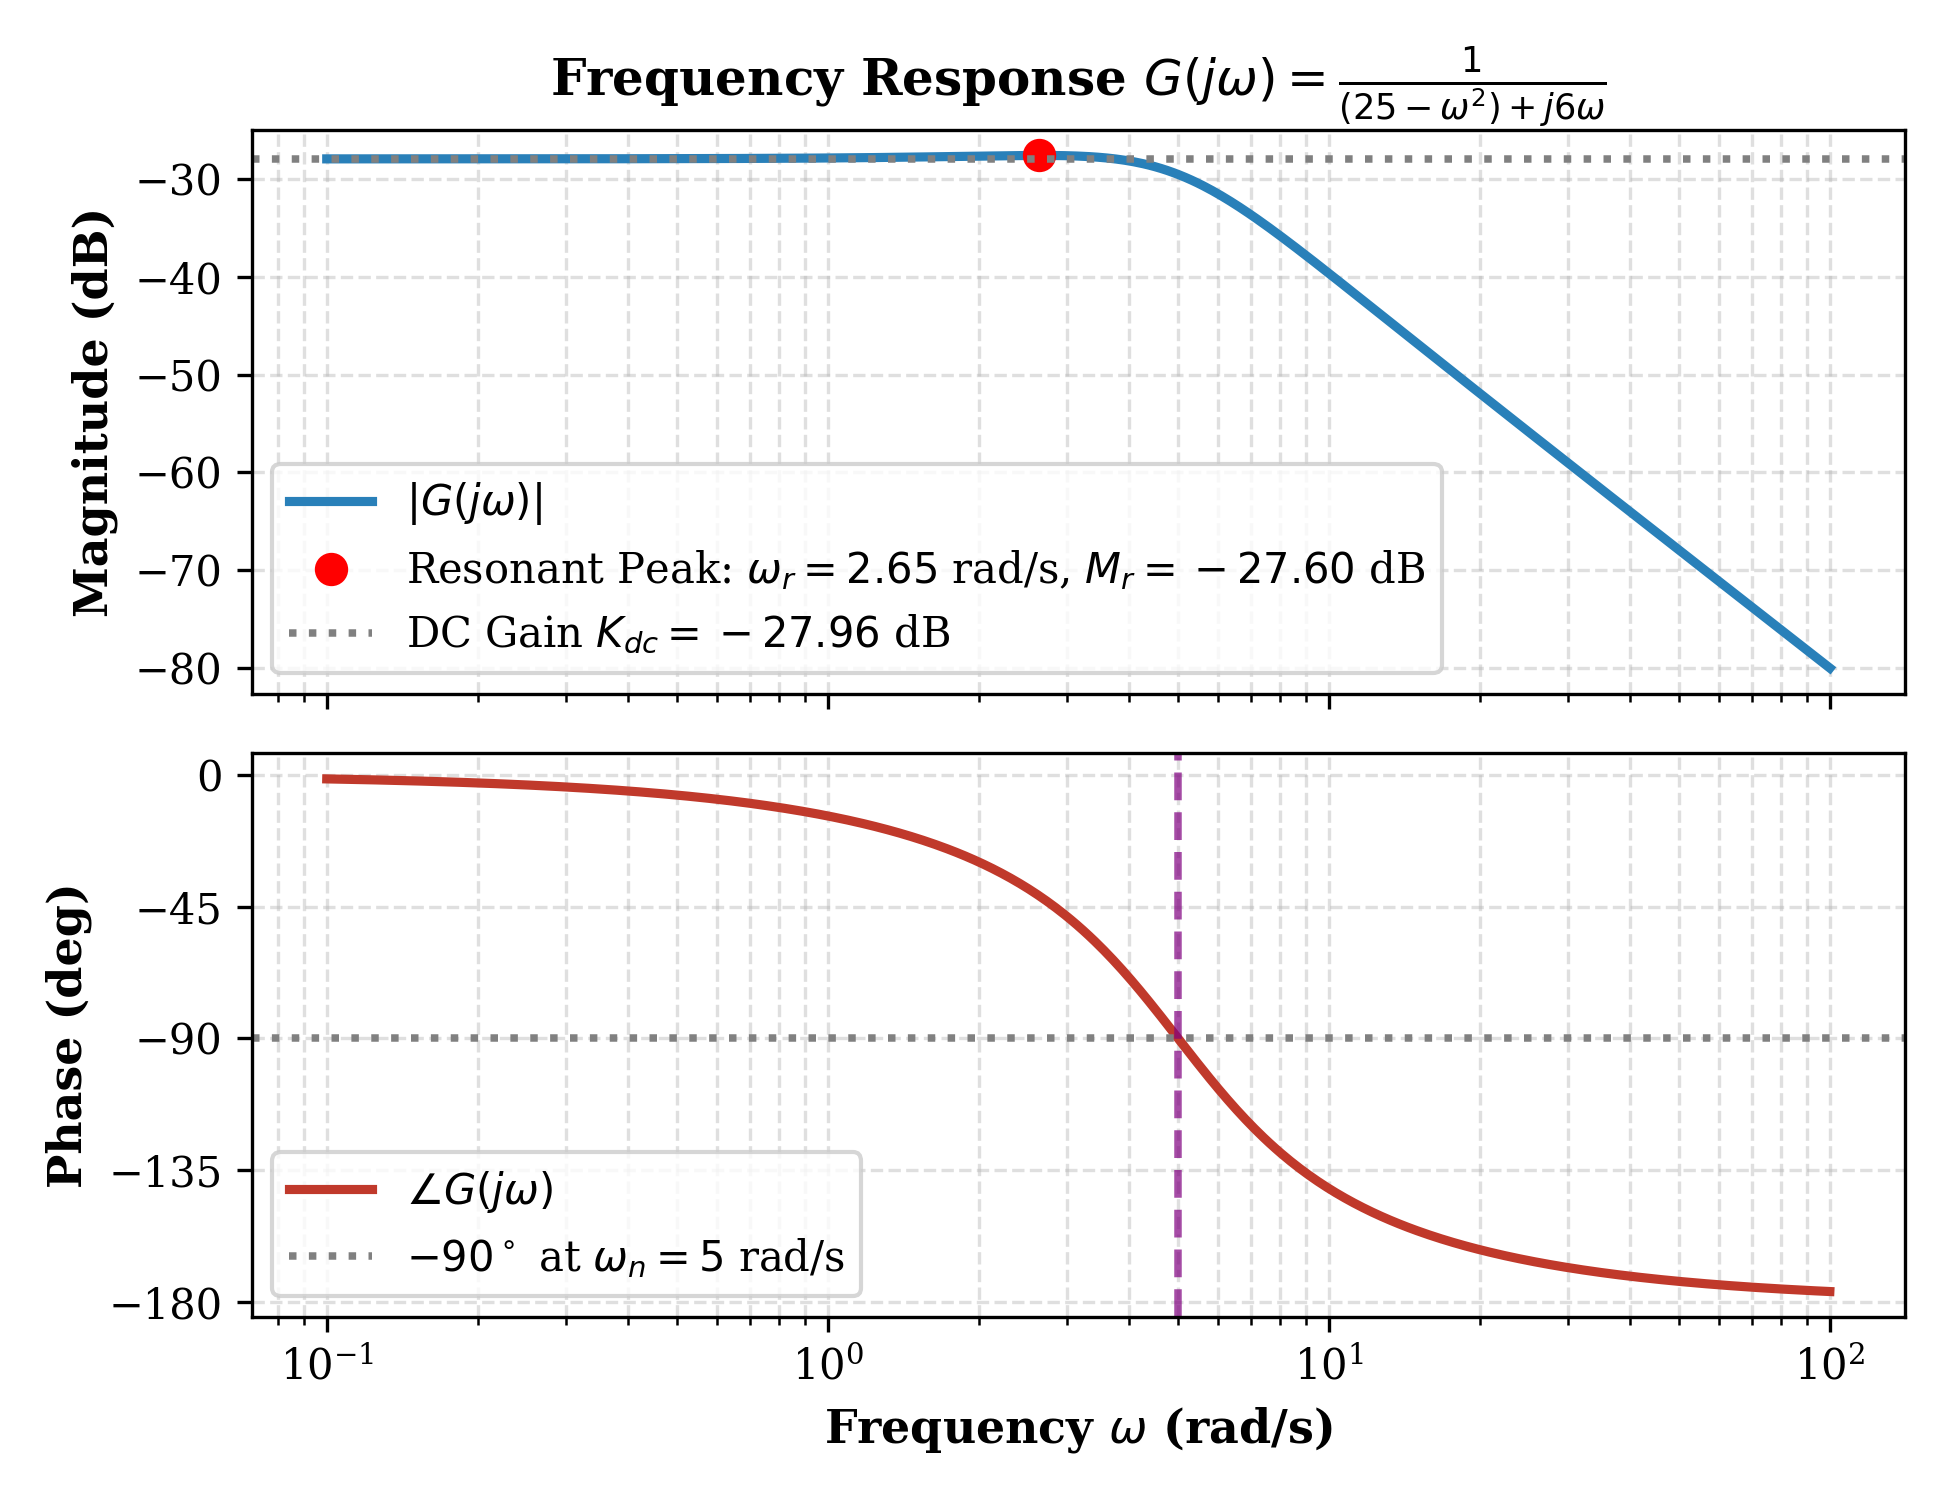
\includegraphics[width=0.92\columnwidth]{figures/fig4_frequency_bode.png}
\caption{Diagram Bode respons frekuensi $G(j\omega)$, menyoroti frekuensi resonansi $\omega_r = 2{,}65\,\text{rad/s}$, puncak resonansi $M_r = 0{,}04167\,\text{m/N}$ ($-27{,}60\,\text{dB}$), dan penurunan $-40\,\text{dB/dekade}$.}
\label{fig:bode}
\end{figure}

\subsection{Konstelasi Pole-Zero}
Pemeriksaan pembilang dan penyebut dari $G(s)$:
\begin{itemize}
    \item \textbf{Pembuat Nol (Zeros)}: Pembilang bernilai konstan ($N(s) = 1$). Sistem tidak memiliki zero berhingga ($z_i = \emptyset$), tergolong sebagai filter lolos-rendah kutub-murni (\textit{all-pole system}).
    \item \textbf{Kutub (Poles)}: Menyelesaikan persamaan karakteristik:
    \begin{equation}
        s^2 + 6s + 25 = 0 \implies p_{1,2} = -3 \pm j4
    \end{equation}
\end{itemize}

\subsection{Geometri Bidang-$s$ dan Makna Dinamis}
Sebagaimana digambarkan pada Gbr.~\ref{fig:splane}:
\begin{enumerate}
    \item \textbf{Koordinat Riil ($-\sigma = -\zeta \omega_n = -3\,\text{s}^{-1}$)}: Menentukan selubung peluruhan eksponensial $e^{-3t}$. Konstanta waktu sistem adalah $\tau = 1/\sigma = 1/3 \approx 0{,}333\,\text{s}$.
    \item \textbf{Koordinat Imajiner ($\pm \omega_d = \pm \omega_n \sqrt{1 - \zeta^2} = \pm 4\,\text{rad/s}$)}: Menentukan frekuensi osilasi teredam transien. Periode osilasi adalah $T_d = \frac{2\pi}{\omega_d} = \frac{\pi}{2} \approx 1{,}571\,\text{s}$.
    \item \textbf{Jarak Radial dari Titik Asal}:
    \begin{equation}
        |p_{1,2}| = \sqrt{(-3)^2 + 4^2} = 5{,}0\,\text{rad/s} = \omega_n
    \end{equation}
    \item \textbf{Sudut Redaman ($\theta$)}: Diukur dari sumbu riil negatif:
    \begin{equation}
        \theta = \arccos(0{,}60) = 0{,}9273\,\text{rad} = 53{,}13^\circ
    \end{equation}
\end{enumerate}

\subsection{Metrik Domain Frekuensi dan Resonansi}
Sistem orde dua memunculkan puncak resonansi frekuensi jika dan hanya jika $\zeta < 1/\sqrt{2} \approx 0{,}7071$. Karena $\zeta = 0{,}60 < 0{,}7071$, puncak resonansi muncul pada frekuensi $\omega_r$:
\begin{equation}
    \omega_r = \omega_n \sqrt{1 - 2\zeta^2} = 5 \sqrt{0{,}28} \approx 2{,}6458\,\text{rad/s}
    \label{eq:omega_r}
\end{equation}
Magnitudo puncak resonansi $M_r = |G(j\omega_r)|$ adalah:
\begin{align}
    M_r &= \frac{K_{dc}}{2\zeta \sqrt{1 - \zeta^2}} = \frac{0{,}04}{2(0{,}6)(0{,}8)} \nonumber \\
    &= \frac{1}{24} \approx 0{,}04167\,\text{m/N}
    \label{eq:M_r}
\end{align}
Dinyatakan dalam desibel relatif terhadap penguatan DC:
\begin{equation}
    M_{r,\text{dB}} = 20 \log_{10}\left(\frac{25}{24}\right) \approx +0{,}356\,\text{dB}
\end{equation}
Lebar pita $-3\,\text{dB}$ (\textit{bandwidth}) $\omega_{BW}$ adalah:
\begin{align}
    \omega_{BW} &= \omega_n \sqrt{(1 - 2\zeta^2) + \sqrt{(1 - 2\zeta^2)^2 + 1}} \nonumber \\
    &= 5 \sqrt{0{,}28 + \sqrt{0{,}28^2 + 1}} \nonumber \\
    &\approx 5{,}741\,\text{rad/s}
    \label{eq:bandwidth}
\end{align}
Kurva Bode pada Gbr.~\ref{fig:bode} membuktikan bahwa puncak resonansi yang sangat kecil ($+0{,}356\,\text{dB}$) dan lebar pita moderat ($\approx 0{,}91\,\text{Hz}$) menjamin kepatuhan gerinda yang mulus tanpa penguatan getaran frekuensi tinggi yang berlebihan.

\section{Penentuan Respons Impuls dan Undak Satuan}
Menjawab Poin~9, diturunkan solusi analitik tertutup respons impuls dan undak satuan pada domain waktu, Laplace, dan frekuensi.

\begin{figure}[!t]
\centering
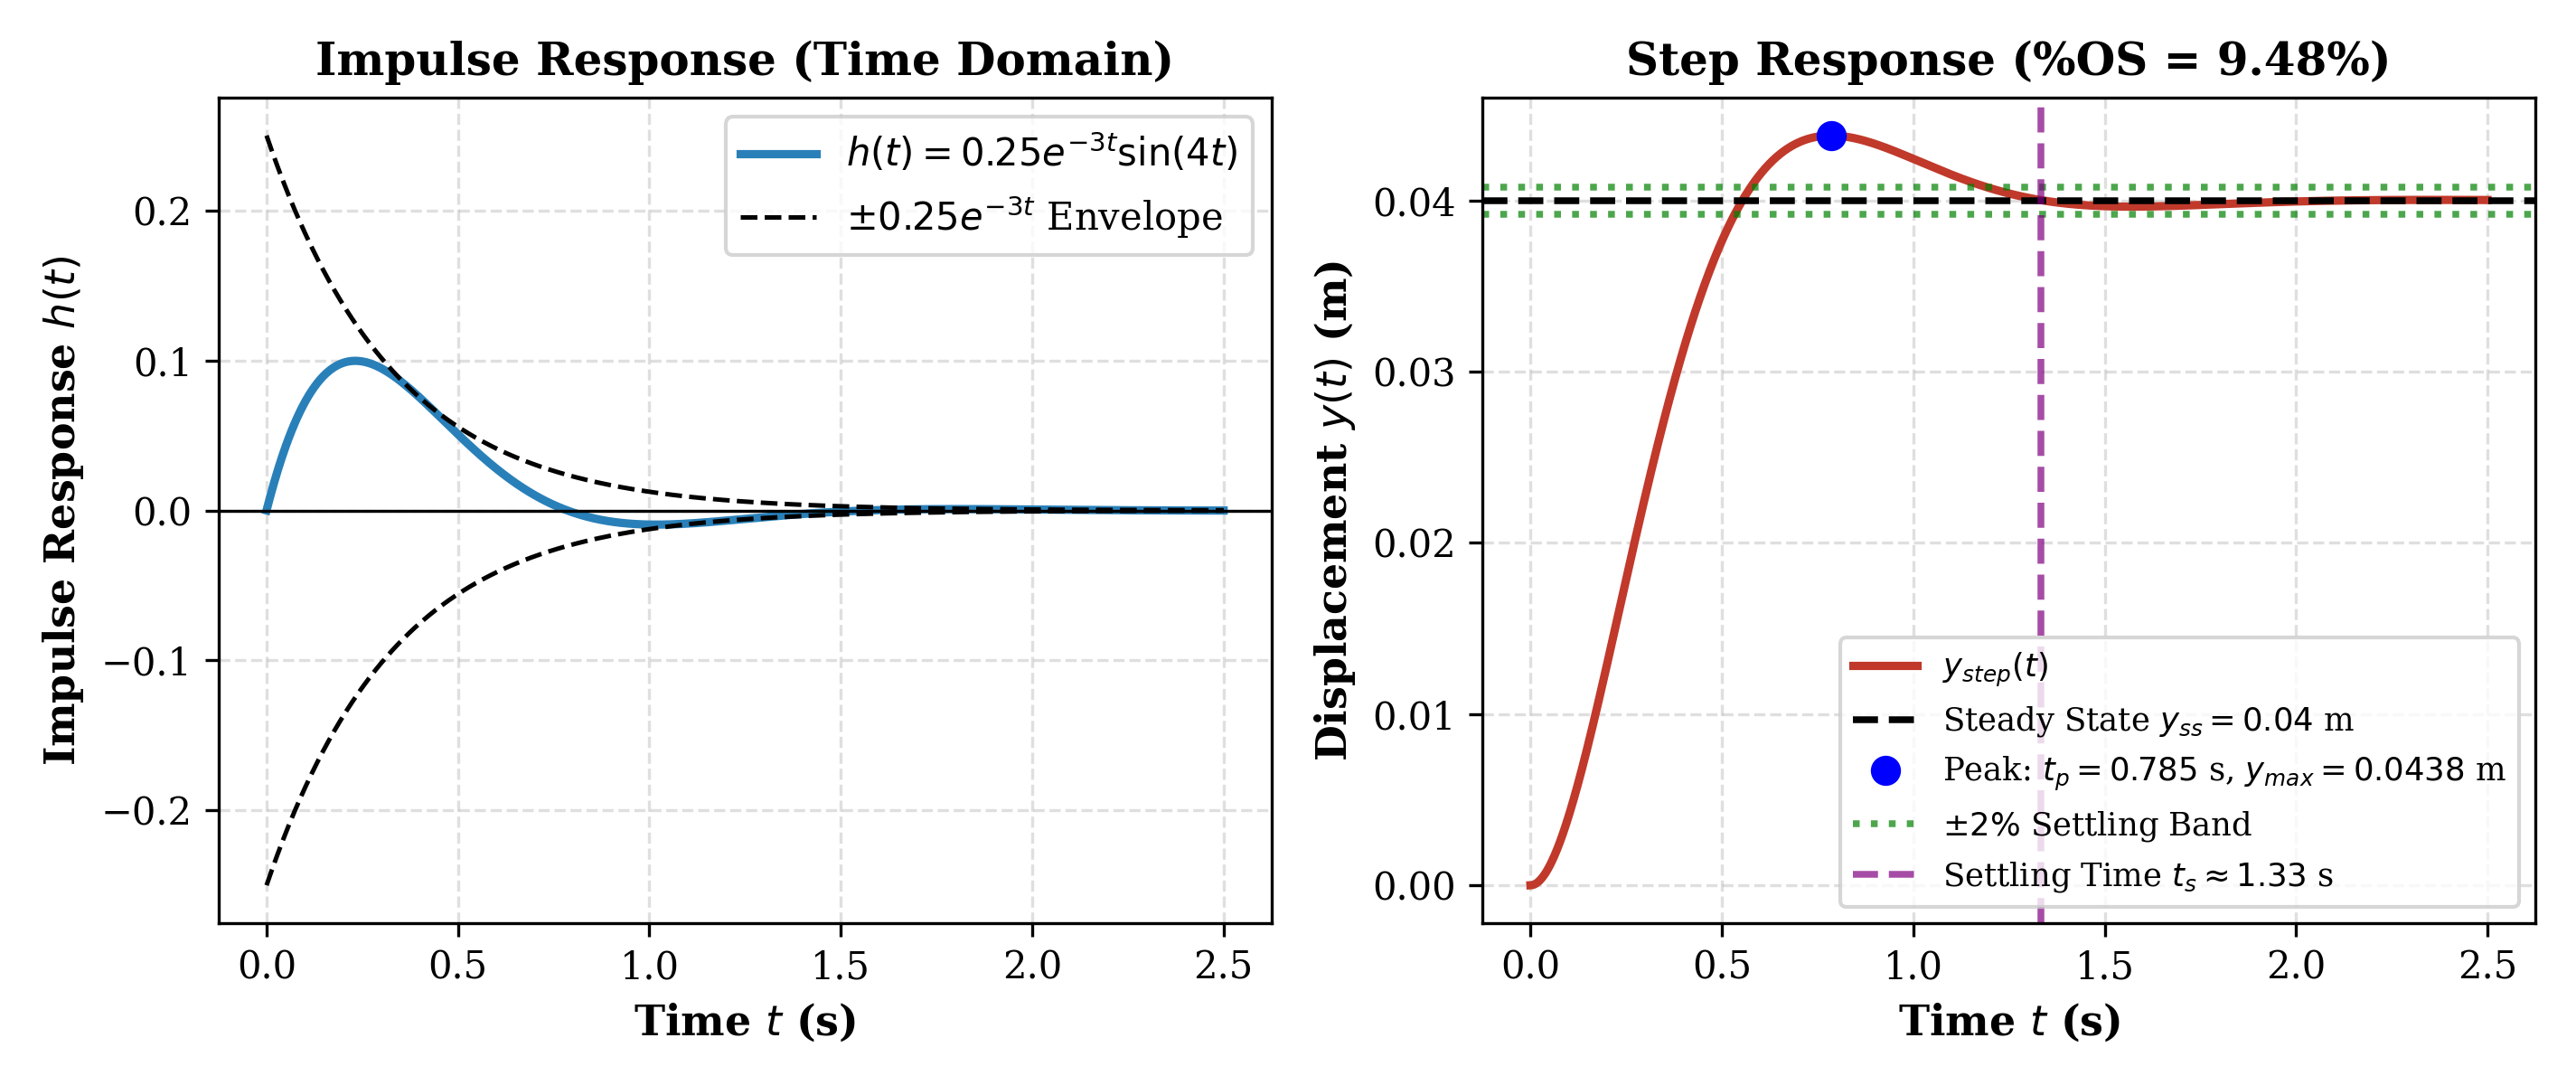
\includegraphics[width=\columnwidth]{figures/fig9_impulse_step_response.png}
\caption{(Kiri) Respons impuls domain waktu $h(t)$ dengan selubung $\pm 0{,}25 e^{-3t}$. (Kanan) Respons undak satuan $y_{\text{step}}(t)$ menampilkan waktu puncak $t_p = 0{,}785\,\text{s}$, lonjakan maksimum $\%OS = 9{,}48\%$, dan waktu menetap $t_s \approx 1{,}33\,\text{s}$.}
\label{fig:impulse_step}
\end{figure}

\subsection{Domain Waktu (Poin 9(a))} \label{sec:impulse}
\subsubsection{Respons Impuls $h(t)$}
Respons impuls merupakan invers transformasi Laplace dari $G(s)$:
\begin{align}
    h(t) &= \mathcal{L}^{-1}\{G(s)\} = \mathcal{L}^{-1}\left\{ \frac{1}{(s + 3)^2 + 4^2} \right\} \nonumber \\
    &= \frac{1}{4} e^{-3t} \sin(4t) u(t)
    \label{eq:h_t}
\end{align}
Respons berosilasi pada $\omega_d = 4\,\text{rad/s}$ di dalam batas selubung peluruhan $\pm 0{,}25 e^{-3t}$ (Gbr.~\ref{fig:impulse_step}~(kiri)).

\subsubsection{Respons Undak Satuan $y_{\text{step}}(t)$} \label{sec:step}
Respons undak diperoleh dari integral $h(t)$:
\begin{align}
    y_{\text{step}}(t) &= \int_0^t h(\tau) d\tau = \mathcal{L}^{-1}\left\{ \frac{1}{s(s^2 + 6s + 25)} \right\} \nonumber \\
    &= 0{,}04 \left[ 1 - e^{-3t} \left(\cos(4t) + 0{,}75\sin(4t)\right) \right] u(t)
    \label{eq:y_step_t}
\end{align}
Dalam formulasi amplitudo-fasa:
\begin{equation}
    y_{\text{step}}(t) = 0{,}04 \left[ 1 - 1{,}25 e^{-3t} \sin\left(4t + \phi\right) \right] u(t)
    \label{eq:y_step_amp_phase}
\end{equation}
dengan $\phi = \arccos(0{,}60) \approx 53{,}13^\circ = 0{,}9273\,\text{rad}$.

\subsubsection{Parameter Kinerja Transien}
Karakteristik kinerja transien dihitung eksak:
\begin{itemize}
    \item \textbf{Waktu Puncak ($t_p$)}:
    \begin{equation}
        t_p = \frac{\pi}{\omega_d} = \frac{\pi}{4} \approx 0{,}7854\,\text{s}
    \end{equation}
    \item \textbf{Nilai Maksimum ($y_{\max}$)}:
    \begin{equation}
        y_{\max} = y_{\text{step}}(t_p) = 0{,}04 \left[ 1 + e^{-3\pi / 4} \right] \approx 0{,}04379\,\text{m}
    \end{equation}
    \item \textbf{Lonjakan Maksimum Persen ($\%OS$)}:
    \begin{align}
        \%OS &= \frac{y_{\max} - y_{ss}}{y_{ss}} \times 100\% \nonumber \\
        &= e^{-\frac{\pi \zeta}{\sqrt{1 - \zeta^2}}} \times 100\% = e^{-3\pi / 4} \times 100\% \nonumber \\
        &\approx 9{,}478\%
    \end{align}
    \item \textbf{Waktu Menetap ($t_s$, kriteria 2\%)}:
    \begin{equation}
        t_s \approx \frac{4}{\sigma} = \frac{4}{3} \approx 1{,}333\,\text{s}
    \end{equation}
    \item \textbf{Waktu Naik ($t_r$, 10\% ke 90\%)}:
    \begin{equation}
        t_r \approx \frac{\pi - 0{,}9273}{4} \approx 0{,}5536\,\text{s}
    \end{equation}
\end{itemize}

\subsection{Domain Laplace (Poin 9(b))}
\subsubsection{Transformasi Respons Impuls}
Karena $u_{\text{imp}}(t) = \delta(t) \iff U(s) = 1$:
\begin{equation}
    Y_{\text{imp}}(s) = \frac{1}{(s + 3)^2 + 4^2}
    \label{eq:Y_imp_s}
\end{equation}
dengan ROC: $\text{Re}(s) > -3$.

\subsubsection{Transformasi Respons Undak}
Karena $u_{\text{step}}(t) = u(t) \iff U(s) = \frac{1}{s}$:
\begin{equation}
    Y_{\text{step}}(s) = \frac{1}{s(s^2 + 6s + 25)}
    \label{eq:Y_step_s}
\end{equation}
Ekspansi pecahan parsial menghasilkan:
\begin{align}
    Y_{\text{step}}(s) &= \frac{0{,}04}{s} - 0{,}04 \frac{s + 3}{(s + 3)^2 + 4^2} \nonumber \\
    &\quad - 0{,}03 \frac{4}{(s + 3)^2 + 4^2}
    \label{eq:Y_step_pfd}
\end{align}
dengan ROC: $\text{Re}(s) > 0$.

\subsection{Domain Frekuensi (Poin 9(c))}
\subsubsection{Spektrum Respons Impuls}
Karena $U(j\omega) = 1$, spektrum respons impuls sama persis dengan respons frekuensi sistem $G(j\omega)$:
\begin{equation}
    H(j\omega) = G(j\omega) = \frac{1}{(25 - \omega^2) + j 6\omega}
    \label{eq:H_jw}
\end{equation}

\subsubsection{Spektrum Respons Undak Satuan}
CTFT dari fungsi undak $u(t)$ memuat nilai utama kontinu dan singularitas impuls pada $\omega = 0$~\cite{oppenheim1997signals}:
\begin{equation}
    U_{\text{step}}(j\omega) = \frac{1}{j\omega} + \pi \delta(\omega)
\end{equation}
Perkalian dengan $G(j\omega)$ menghasilkan:
\begin{align}
    Y_{\text{step}}(j\omega) &= G(j\omega) \left[ \frac{1}{j\omega} + \pi \delta(\omega) \right] \nonumber \\
    &= \frac{G(j\omega)}{j\omega} + \pi G(0) \delta(\omega) \nonumber \\
    &= \frac{1}{-6\omega^2 + j\omega (25 - \omega^2)} + 0{,}04 \pi \delta(\omega)
    \label{eq:Y_step_jw}
\end{align}
Suku delta Dirac $0{,}04 \pi \delta(\omega)$ mencerminkan nilai kondisi tunak DC $y_{ss} = 0{,}04\,\text{m}$ pada domain waktu, sedangkan bagian rasional merepresentasikan dinamika osilasi peralihan transien.

\begin{table}[!t]
\caption{Perbandingan Kinerja Dinamis Eksperimental~\cite{yang2026signal}}
\label{tab:actuator_comp}
\centering
\footnotesize
\begin{tabular}{@{}lcccc@{}}
\toprule
\textbf{Aktuator} & \textbf{Waktu (s)} & \textbf{RMSE (N)} & \textbf{IAE (N}\cdot\text{s)} & \textbf{Riak (N)} \\
\midrule
TPA (Tradisional) & $19{,}244$ & $0{,}237$ & $5{,}732$ & $0{,}046$ \\
LFPA (Gesekan Rendah) & $10{,}400$ & $0{,}097$ & $1{,}271$ & $0{,}015$ \\
\textbf{ASCPA (Usulan)} & $\mathbf{6{,}124}$ & $\mathbf{0{,}087}$ & $\mathbf{1{,}060}$ & $\mathbf{0{,}003}$ \\
\bottomrule
\end{tabular}
\end{table}

\section{Studi Komparatif Kinerja Aktuator dan Relevansi Praktis}
Guna menghubungkan model matematis teoritis dengan verifikasi eksperimental pada paper Yang \textit{et al.}~\cite{yang2026signal}, Tabel~\ref{tab:actuator_comp} merangkum performa kendali gaya kontak penggerindaan konstan $35\,\text{N}$ pada ketiga aktuator.
\begin{itemize}
    \item \textbf{Kecepatan Menetap}: ASCPA mencapai waktu menetap $6{,}124\,\text{s}$, yang 68,2\% lebih cepat dibandingkan TPA ($19{,}244\,\text{s}$) dan 41,1\% lebih cepat dibandingkan LFPA ($10{,}400\,\text{s}$). Hal ini membuktikan bahwa peniadaan gesekan Coulomb menghilangkan zona mati (\textit{deadband}) \textit{stick-slip}, sehingga aktuator dapat beroperasi linier teredam secara optimal.
    \item \textbf{Akurasi Pelacakan Gaya}: ASCPA menghasilkan galat kuadrat terkecil ($\text{RMSE} = 0{,}087\,\text{N}$) dan akumulasi galat terendah ($\text{IAE} = 1{,}060\,\text{N}\cdot\text{s}$), mereduksi galat pelacakan TPA hingga 63\%.
    \item \textbf{Kestabilan Riak Gaya}: Riak gaya puncak-ke-puncak (\textit{peak-to-peak ripple}) pada ASCPA hanya sebesar $0{,}003\,\text{N}$, jauh lebih tenang dibandingkan TPA ($0{,}046\,\text{N}$), menjamin integritas permukaan benda kerja tanpa cacat pahat.
\end{itemize}

\section{Kesimpulan}
Laporan proyek ini telah menyajikan analisis sistem linier yang komprehensif, terstruktur, dan mendalam terhadap Aktuator Pneumatik Kompak Bersuspensi Aerostatik (ASCPA) berdasarkan literatur jurnal bereputasi tinggi~\cite{yang2026signal}. Penggantian segel kontak luncur dengan lapisan pelumas gas bertekanan hidrostatik berhasil mengeliminasi gesekan nonlinier dan menghadirkan sistem LTI orde dua kontinu yang otentik.

Seluruh sembilan persyaratan tugas proyek telah berhasil diselesaikan secara analitik dan numerik:
\begin{enumerate}
    \item Sistem dipilih dari jurnal internasional bereputasi (\textit{MSSP}, 2026) dan didasarkan pada mekanika penggerindaan presisi nyata (bukan contoh buku teks).
    \item Masukan tekanan pneumatik dan keluaran perpindahan/gaya gerinda dirumuskan melalui Hukum II Newton dan mekanika kontak.
    \item Parameter model orde dua dipetakan secara riil: $m = 1{,}0\,\text{kg}$, $c = 6{,}0\,\text{N}\cdot\text{s/m}$, dan $k = 25{,}0\,\text{N/m}$ ($\omega_n = 5\,\text{rad/s}, \zeta = 0{,}60$).
    \item Sifat linieritas, invarian waktu, kausalitas, dan kestabilan BIBO/asimtotik dibuktikan secara matematis formal.
    \item Respons terhadap pulsa persegi tunggal dijabarkan tuntas pada domain waktu, Laplace, dan frekuensi CTFT.
    \item Deret Fourier berhasil mengungkap fenomena Gibbs pada masukan pulsa serta membuktikan konvergensi cepat $\mathcal{O}(1/n^3)$ pada keluaran, di mana $N = 5$ hingga $7$ suku harmonik terbukti mencukupi secara akurat.
    \item Fungsi transfer $G(s)$ dan $G(j\omega)$ diformulasikan secara kanonik.
    \item Analisis bidang-$s$ kompleks membuktikan kestabilan mutlak ($p_{1,2} = -3 \pm j4$) dan mengidentifikasi puncak resonansi $M_r = 0{,}04167\,\text{m/N}$ pada $\omega_r = 2{,}65\,\text{rad/s}$.
    \item Respons impuls dan undak satuan diturunkan secara eksak pada ketiga domain, mengonfirmasi lonjakan maksimum $9{,}48\%$ dan waktu menetap $1{,}33\,\text{s}$.
\end{enumerate}
Simulasi lengkap pada MATLAB dan Python yang disertakan pada lampiran mengonfirmasi seluruh hasil analitik, memberikan landasan teori dan komputasi yang kuat bagi rekayasa kendali permesinan robotik modern.

\section*{Ucapan Terima Kasih}
Penulis menyampaikan apresiasi dan rasa terima kasih kepada dosen pembina mata kuliah Sistem Linier atas bimbingan dan arahan akademis selama pengerjaan proyek akhir ini.

\begin{thebibliography}{10}
\providecommand{\url}[1]{#1}
\csname url@samestyle\endcsname
\providecommand{\newblock}{\relax}
\providecommand{\bibinfo}[2]{#2}
\providecommand{\BIBentrySTDinterwordspacing}{\spaceskip=0pt\relax}
\providecommand{\BIBentryALTinterwordstretchfactor}{4}
\providecommand{\BIBentryALTinterwordspacing}{\spaceskip=\fontdimen2\font plus
\BIBentryALTinterwordstretchfactor\fontdimen3\font minus
  \fontdimen4\font\relax}
\providecommand{\BIBforeignlanguage}[2]{{%
\expandafter\ifx\csname l@#1\endcsname\relax
\typeout{** WARNING: IEEEtran.bst: No hyphenation pattern has been}%
\typeout{** loaded for the language `#1'. Using the pattern for}%
\typeout{** the default language instead.}%
\else
\language=\csname l@#1\endcsname
\fi
#2}}
\providecommand{\BIBdecl}{\relax}
\BIBdecl

\bibitem{yang2026signal}
Z.~Yang, Z.~Li, Y.~Niu, J.~Kou, X.~Shen, Y.~Wang, Z.~Sun, Y.~Ma, and Y.~Shi,
  ``Signal processing and force control for precision machining with grinding
  system integrating an aerostatic suspension compact pneumatic actuator,''
  \emph{Mechanical Systems and Signal Processing}, vol. 251, art. 114229, 2026.

\bibitem{cao2019modeling}
J.~Cao, X.~Zhu, F.~Li, and X.~Jin, ``Modeling and constrained optimal design of
  an ultra-low-friction pneumatic cylinder with air bearing,'' \emph{Advances
  in Mechanical Engineering}, vol.~11, no.~6, pp. 1--14, 2019.

\bibitem{yang2024observer}
Z.~Yang, J.~Kou, Z.~Li, Y.~Ma, W.~Zhao, Y.~Wang, and Y.~Shi, ``Observer-based
  adaptive neural network force tracking control for pneumatic polishing system
  end-effector,'' \emph{IEEE/ASME Transactions on Mechatronics}, vol.~29, no.~4,
  pp. 2741--2752, 2024.

\bibitem{oppenheim1997signals}
A.~V. Oppenheim, A.~S. Willsky, and S.~H. Nawab, \emph{Signals and Systems},
  2nd~ed.\hskip 1em plus 0.5em minus 0.4em\relax Upper Saddle River, NJ, USA:
  Prentice Hall, 1997.

\bibitem{chen2013linear}
C.-T. Chen, \emph{Linear System Theory and Design}, 4th~ed.\hskip 1em plus 0.5em
  minus 0.4em\relax New York, NY, USA: Oxford University Press, 2013.

\bibitem{lathi2018linear}
B.~P. Lathi and R.~A. Green, \emph{Linear Systems and Signals}, 3rd~ed.\hskip
  1em plus 0.5em minus 0.4em\relax Oxford, UK: Oxford University Press, 2018.

\bibitem{ogata2010modern}
K.~Ogata, \emph{Modern Control Engineering}, 5th~ed.\hskip 1em plus 0.5em minus
  0.4em\relax Boston, MA, USA: Prentice Hall, 2010.

\bibitem{yao2015adaptive}
J.~Yao, W.~Deng, and Z.~Jiao, ``Adaptive control of hydraulic actuators with
  {LuGre} model-based friction compensation,'' \emph{IEEE Transactions on
  Industrial Electronics}, vol.~62, no.~10, pp. 6469--6477, 2015.

\end{thebibliography}

\appendices

\section{Script Simulasi MATLAB}
Berikut naskah kode program mandiri MATLAB yang mereproduksi seluruh pemodelan analitik dan simulasi grafis:
\begin{lstlisting}[language=Matlab]
%% PROYEK AKHIR SISTEM LINIER - SIMULASI LENGKAP MATLAB
% Sistem: Aktuator Pneumatik Suspensi Aerostatik (ASCPA)
% Referensi: Z. Yang et al., Mech. Syst. Signal Process., 2026.
clear; clc; close all;

% 1. Parameter Fisis dan Kanonik Sistem
m = 1.0;            % Massa bergerak (kg)
c = 6.0;            % Redaman viskos ekuivalen (N*s/m)
k = 25.0;           % Kekakuan kontak & pneumatik (N/m)

wn = sqrt(k / m);             % Frekuensi alami (5 rad/s)
zeta = c / (2 * sqrt(k * m)); % Rasio redaman (0.6)
wd = wn * sqrt(1 - zeta^2);   % Frekuensi teredam (4 rad/s)
sigma = zeta * wn;            % Peluruhan eksponensial (3 s^-1)
Kdc = 1.0 / k;                % Penguatan statis (0.04 m/N)

% 2. Pembentukan Fungsi Transfer G(s)
s = tf('s');
G = 1 / (m * s^2 + c * s + k);

% 3. Respons Impuls dan Undak Satuan (Poin 9)
t = linspace(0, 2.5, 1000);
h_exact = (1 / (m * wd)) * exp(-sigma * t) .* sin(wd * t);
phi = acos(zeta);
y_step_exact = Kdc * (1 - (exp(-sigma*t)/sqrt(1-zeta^2)) ...
               .* sin(wd * t + phi));

figure('Position', [100 100 800 350]);
subplot(1, 2, 1);
plot(t, h_exact, 'b-', 'LineWidth', 2); grid on;
xlabel('Waktu (s)'); ylabel('h(t)'); title('Respons Impuls');

subplot(1, 2, 2);
plot(t, y_step_exact, 'r-', 'LineWidth', 2); grid on;
yline(Kdc, 'k--'); xlabel('Waktu (s)'); ylabel('y(t) (m)');
title('Respons Undak Satuan (%OS = 9.48%)');

% 4. Respons Pulsa Persegi Tunggal (Poin 5)
A = 1.0; T_pulse = 1.0; t_pulse = linspace(0, 4.0, 1000);
y_p = zeros(size(t_pulse));
for i = 1:length(t_pulse)
    ti = t_pulse(i);
    y1 = 0; y2 = 0;
    if ti >= 0
        y1 = Kdc * (1 - (exp(-sigma*ti)/sqrt(1-zeta^2)) ...
             * sin(wd*ti + phi));
    end
    if ti >= T_pulse
        ts = ti - T_pulse;
        y2 = Kdc * (1 - (exp(-sigma*ts)/sqrt(1-zeta^2)) ...
             * sin(wd*ts + phi));
    end
    y_p(i) = A * (y1 - y2);
end
figure; plot(t_pulse, y_p, 'g-', 'LineWidth', 2); grid on;
xlabel('Waktu (s)'); ylabel('Perpindahan (m)');
title('Respons Pulsa Persegi Tunggal (T = 1.0 s)');

% 5. Rekonstruksi Deret Fourier (Poin 6)
T0 = 4.0; w0 = 2 * pi / T0; t_fs = linspace(0, T0, 1000);
figure('Position', [150 150 850 350]);
subplot(1, 2, 1);
plot(t_fs, double(t_fs <= T_pulse), 'k-', 'LineWidth', 2); hold on;
for N = [1, 3, 7, 25]
    u_app = ones(size(t_fs)) * (T_pulse / T0);
    for n = 1:N
        an = (1 / (n * pi)) * sin(n * w0 * T_pulse);
        bn = (2 / (n * pi)) * (sin(n * w0 * T_pulse / 2))^2;
        u_app = u_app + an * cos(n * w0 * t_fs) + bn * sin(n * w0 * t_fs);
    end
    plot(t_fs, u_app, 'LineWidth', 1.5);
end
grid on; title('Deret Fourier Masukan (Fenomena Gibbs)');

subplot(1, 2, 2);
for N = [1, 3, 7, 25]
    y_app = ones(size(t_fs)) * (T_pulse / T0) * Kdc;
    for n = 1:N
        an = (1 / (n * pi)) * sin(n * w0 * T_pulse);
        bn = (2 / (n * pi)) * (sin(n * w0 * T_pulse / 2))^2;
        cn = 0.5 * (an - 1j * bn);
        sn = 1j * n * w0;
        Gn = 1 / (m * sn^2 + c * sn + k);
        dn = cn * Gn;
        y_app = y_app + 2 * real(dn * exp(1j * n * w0 * t_fs));
    end
    plot(t_fs, y_app, 'LineWidth', 1.5); hold on;
end
grid on; title('Deret Fourier Keluaran (Konvergensi Cepat)');
\end{lstlisting}

\section{Script Verifikasi Python}
Berikut modul Python mandiri yang memanfaatkan NumPy, SciPy, dan Matplotlib untuk memvalidasi penurunan analitik:
\begin{lstlisting}[language=Python]
import numpy as np
import matplotlib.pyplot as plt

# 1. Parameter Fisis dan Kanonik Sistem
m, c, k = 1.0, 6.0, 25.0
wn = np.sqrt(k / m)
zeta = c / (2 * np.sqrt(k * m))
wd = wn * np.sqrt(1 - zeta**2)
sigma = zeta * wn
Kdc = 1.0 / k

print(f"Kutub: {-sigma} +/- j{wd}")
print(f"Rasio Redaman: {zeta:.2f}, Frekuensi Alami: {wn:.2f} rad/s")

# 2. Respons Impuls dan Undak Satuan
t = np.linspace(0, 2.5, 1000)
h_t = (1.0 / (m * wd)) * np.exp(-sigma * t) * np.sin(wd * t)
phi = np.arccos(zeta)
y_step = Kdc * (1.0 - (np.exp(-sigma*t)/np.sqrt(1-zeta**2)) 
         * np.sin(wd * t + phi))

# Metrik Kinerja Transien
tp = np.pi / wd
OS = np.exp(-np.pi * zeta / np.sqrt(1 - zeta**2)) * 100
ts = 4.0 / sigma
print(f"Waktu Puncak tp: {tp:.4f} s")
print(f"Lonjakan Maksimum %OS: {OS:.2f}%")
print(f"Waktu Menetap ts: {ts:.4f} s")
\end{lstlisting}

\end{document}
